\documentclass{beamer}

\mode<presentation> {
	\usetheme{Boadilla}
}
\usefonttheme[onlymath]{serif}
\usepackage{graphicx} % Allows including images
\usepackage{booktabs} % Allows the use of \toprule, \midrule and \bottomrule in tables
\usepackage{amsmath}
\usepackage{amsfonts}
\usepackage{enumerate}
\usepackage{color}
%----------------------------------------------------------------------------------------

\title[JPE, 2020]{Willingness to Pay for Clean Air \\ {\small Evidence from Air Purifier Markets in China}}

\author{Koichiro Ito, Shuang Zhang} 
\institute[]{Presenter: Qinzhu Sun}

\date{\today} % Date, can be changed to a custom date
\logo{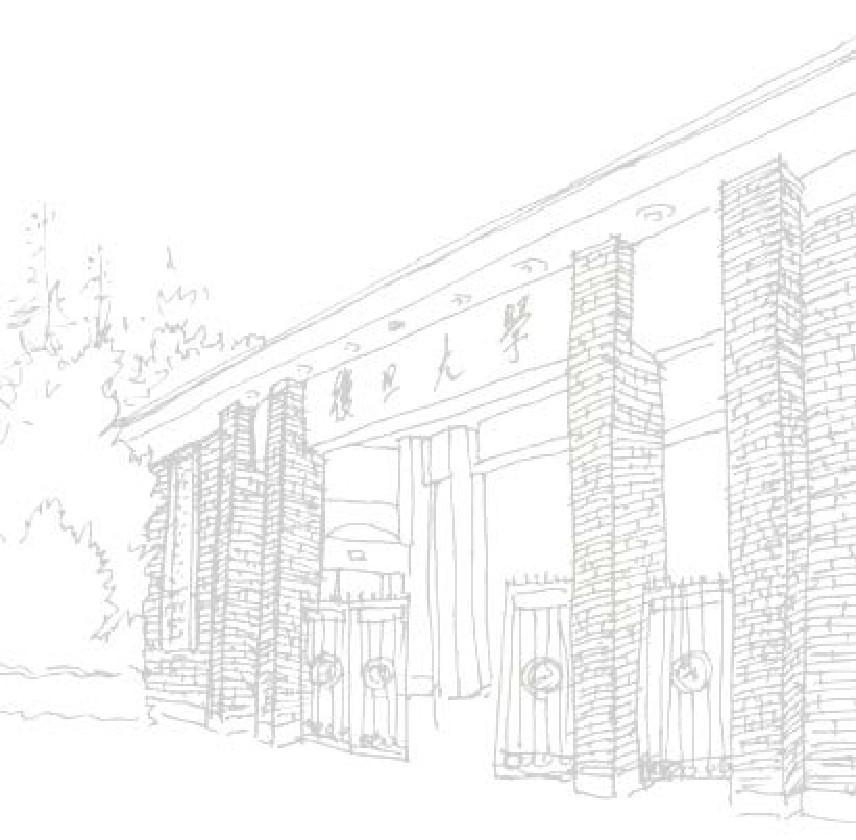
\includegraphics[scale=0.2]{maingate2}}
\begin{document}

\begin{frame}
\titlepage
\end{frame}

\begin{frame}{Overview}
\tableofcontents
\end{frame}
%------------------------------------------------

%------------------------------------------------
\section{Introduction}
\begin{frame}[shrink]
	\transfade %fade in and fade out
	\tableofcontents[sectionstyle=show/shaded,subsectionstyle=show/shaded/hide]
	\addtocounter{framenumber}{-1}
\end{frame}
%------------------------------------------------
\begin{frame}{About the authors}
	\begin{columns}
		\column{0.7\textwidth}
		\textbf{Koichiro Ito} 
		\begin{itemize}
			\item Associate Professor at Harris School of Public Policy, University of Chicago
			\item Research interest: Energy Economics, Environmental Economics, Industrial Organization, Public Economics
			\item Publication: AER(2), JPE, AEJ(2), REStat\dots
		\end{itemize}
		\textbf{Shuang Zhang} 
		\begin{itemize}
			\item Associate Professor of Economics, University of Colorado Boulder and NBER (on leave 2020-2021)
			\item Research interest: Environment and Energy, Health, Development, China
			\item Publication: JPE(2), JDE, PNAS, EDCC\dots
		\end{itemize}
		\column{0.3\textwidth}
		
\includegraphics[width=2.5cm]{ito.jpg}
		
\includegraphics[width=2.5cm]{zhang.jpg}
	\end{columns}
\end{frame}
%------------------------------------------------
\begin{frame}{Introduction}
	\begin{itemize}
		\item Air pollution causes negative impacts on various economic outcomes, including infant mortality, life expectancy, and labor supply.
		\item However, a great economic burden of air pollution does not necessarily imply that existing environmental regulations are not optimal.
		\item [-] Optimal environmental regulation depends on the extent to which individuals value air quality improvements—that is, their willingness to pay (WTP) for clean air (Greenstone and Jack 2013).
		\item [-] Obtaining a revealed-preference estimate of WTP for clean air
		is challenging in developing countries because of limited data and a lack of readily available exogenous variation in air quality.
	\end{itemize}
\end{frame}
%------------------------------------------------
\begin{frame}{Introduction}
	\begin{itemize}
		\item This paper provides among the first revealed-preference estimates of WTP for clean air in developing countries.
		\item Idea: Demand for home-use air purifiers provides valuable information	for the estimation of WTP for air quality improvements.
	\end{itemize}
\end{frame}
%------------------------------------------------

%------------------------------------------------
\section{Air Pollution, Air Purifiers \& Huai River Policy}
\begin{frame}[shrink]
	\transfade %fade in and fade out
	\tableofcontents[sectionstyle=show/shaded,subsectionstyle=show/shaded/hide]
	\addtocounter{framenumber}{-1}
\end{frame}
%------------------------------------------------
\begin{frame}{Air Pollution, Air Purifiers \& Huai River Policy}{A. Air Purifiers}
	\begin{itemize}
		\item A key advantage of analyzing air purifier markets is that one of the product attributes—HEPA—informs both consumers and econometricians about the purifier’s effectiveness at reducing indoor particulate matter.
		\item [-] A HEPA air purifier removes at least 99.97\% of particles that are 0.3 mm or larger in diameter.
		\item [-] In contrast, non-HEPA purifiers are not effective at reducing small particles, such as PM2.5 and PM10. Yet non-HEPA purifiers provide consumers utility gains through attributes other than HEPA because these attributes are effective in removing other indoor pollutants.
	\end{itemize}
\end{frame}
%------------------------------------------------
\begin{frame}{Air Pollution, Air Purifiers \& Huai River Policy}{B. Huai River Policy and Its Recent Reform}
	\begin{itemize}
		\item The government provided citywide centralized heating to northern cities only (Almond et al. 2009). Northern and southern China are divided by a line formed by the Huai River and Qinling Mountains. The government used this line because the average January temperature is roughly 0$^\circ$C along the line and the line is not a border for other administrative purposes (Chen et al. 2013).
		\item In July 2003, the Chinese government issued a heating reform, which changed the payment system from free provision to flat-rate billing (World Bank 2005).
		\item Our analysis focuses on the period from 2006 to 2014, after the 2003 reform on heating billing.
	\end{itemize}
\end{frame}
%------------------------------------------------
\begin{frame}{Air Pollution, Air Purifiers \& Huai River Policy}{B. Huai River Policy and Its Recent Reform}
	\centering
	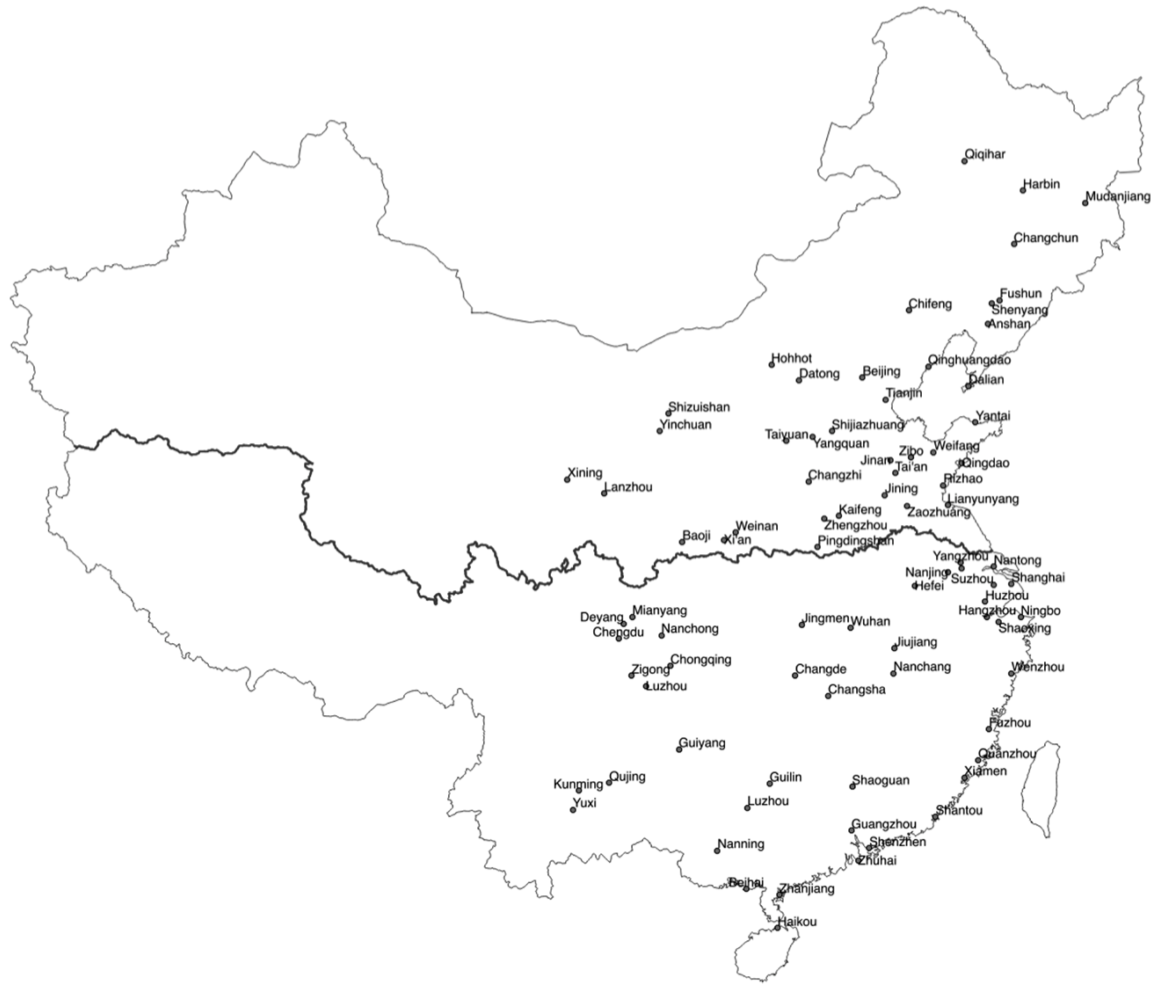
\includegraphics[scale=0.6]{figure1.png}
\end{frame}
%------------------------------------------------

%------------------------------------------------
\section{Data \& Descriptive Statistics}
\begin{frame}[shrink]
	\transfade %fade in and fade out
	\tableofcontents[sectionstyle=show/shaded,subsectionstyle=show/shaded/hide]
	\addtocounter{framenumber}{-1}
\end{frame}
%------------------------------------------------
\begin{frame}{Data}{Air Purifier Data}
	\begin{itemize}
		\item This paper uses air purifier sales transaction data collected by a marketing firm in China (2006 - 2014) for 80 cities. Provided are monthly sales and monthly average price for each product by store, along with information on product attributes.
		\item [-] The data set covers in-store transactions in major department stores and electrical appliance stores, accounting for over 80\% of all in-store sales.
		\item [-] During the period 2006–14, in-store sales made up 72\% of overall purifier sales (including in-store and online sales).
	\end{itemize}
\end{frame}
%------------------------------------------------
\begin{frame}{Data}{Air Purifier Data}
	\begin{itemize}
		\item Because our data set does not cover 100\% of purifier sales, we take \textbf{two approaches to defining sales volume}.
		\item [-] In the first approach, we simply ignore transactions outside the data set $\Rightarrow$ underestimate the sales volume;
		\item [-] In the second approach, we adjust sales volume proportionally to address this limitation. Specifically, we multiply the sales volume of each product by 1.73 ($=1/(0.8\cdot0.72)$).
		\bigskip
		\item We aggregate the transaction data to the product-city level.
	\end{itemize}
\end{frame}
%------------------------------------------------
\begin{frame}{Data}{Air Pollution / Demographic / GIS Data}
	\begin{itemize}
		\item \textbf{Air Pollution Data:} city-level annual average PM$_{10}$ from 2006 to 2014 (Ebenstein et al., 2017).
		\item [-] {\small Source: \textit{China's Environmental Yearbooks}; \textit{China's Environmental Quality Annual Reports}.}
		\item \textbf{Demographic Data:} city-year measures on population, urban population, and GDP per capita; individual-level microdata (income, education, housing)
		\item [-] {\small Source: City Statistical Yearbooks in 2006–14; 2005 census}
		\item \textbf{GIS Data \& Map:} construct two distance variables
		\item [-] Distance between a city and the Huai River;
		\item [-] Road distance from a city’s centroid to the factory or importing port locations of air purifiers.
	\end{itemize}
\end{frame}
%------------------------------------------------
\begin{frame}{Summary Statistics and Testing for Balance in Observables}
	\centering
	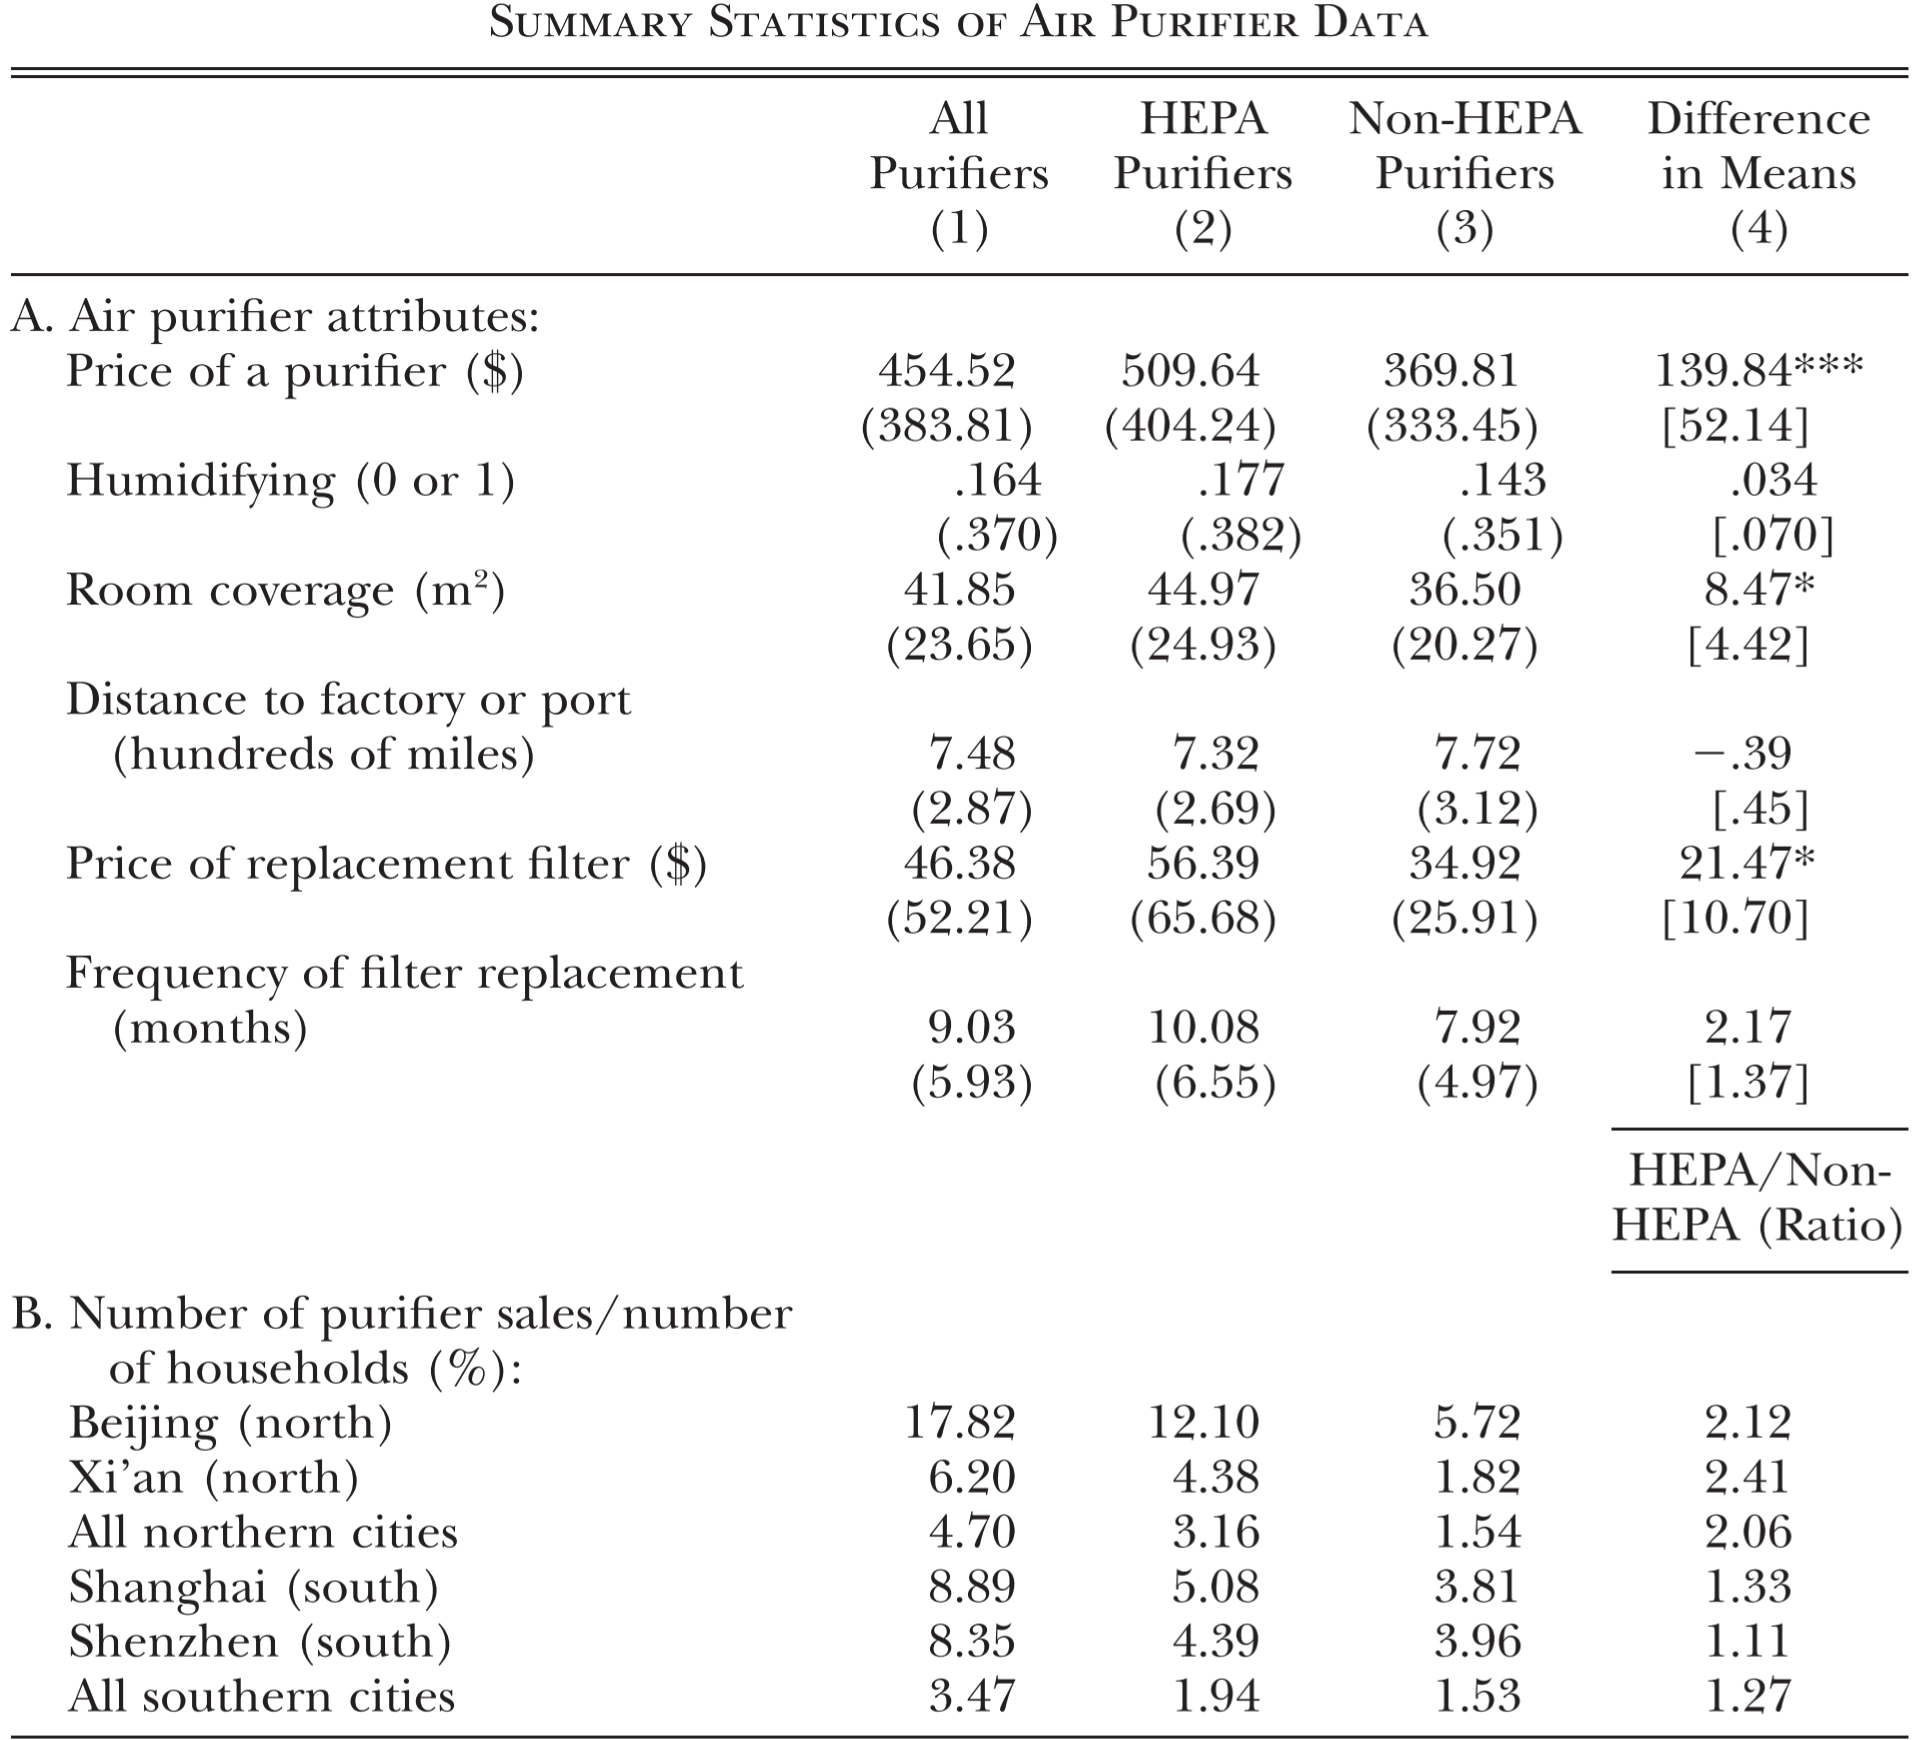
\includegraphics[scale=0.35]{table1.png}
\end{frame}
%------------------------------------------------
\begin{frame}[label=balancetest]{Summary Statistics and Testing for Balance in Observables}
	\centering
	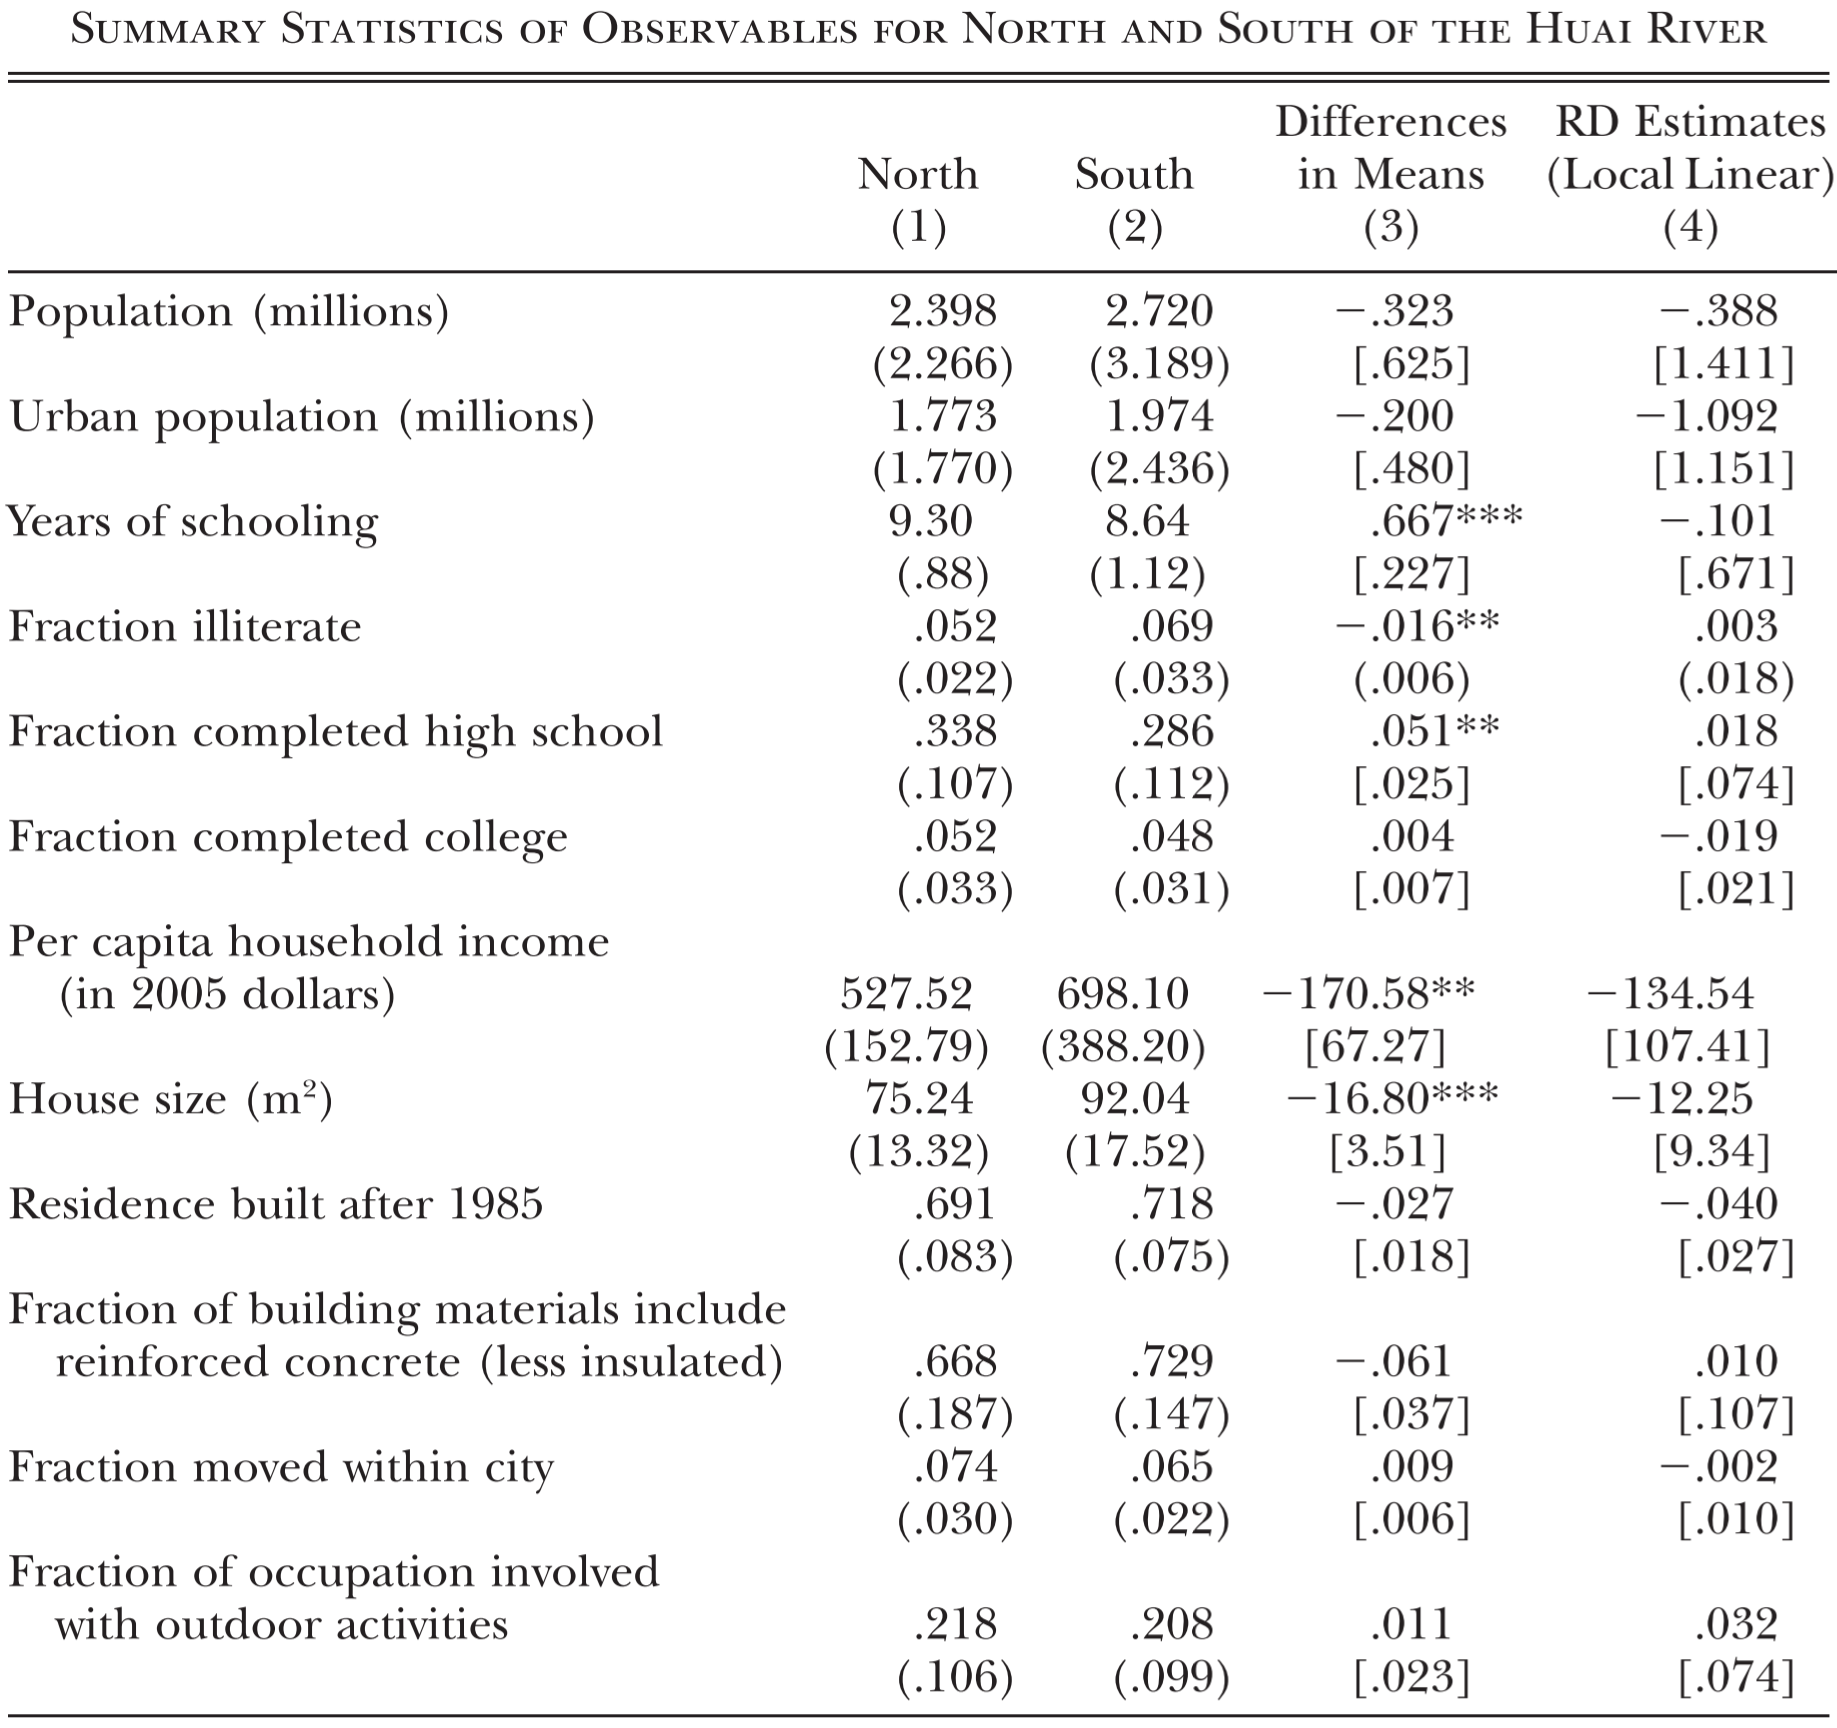
\includegraphics[scale=0.35]{table2.png}
\end{frame}
%------------------------------------------------

%------------------------------------------------
\section{Demand for Air Purifiers}
\begin{frame}[shrink]
	\transfade %fade in and fade out
	\tableofcontents[sectionstyle=show/shaded,subsectionstyle=show/shaded/hide]
	\addtocounter{framenumber}{-1}
\end{frame}
%------------------------------------------------
\begin{frame}{Random-Utility Model}
	\begin{itemize}
		\item Our goal is to obtain a revealed-preference estimate of WTP for clean air by analyzing demand for air purifiers. Because air purifiers are differentiated products, start with a random-utility model.
		\item Intuition: the extent to which consumers value this characteristic, along with the price elasticity of demand, provides useful information on their WTP for indoor air quality improvements.
	\end{itemize}
	The \textbf{indirect utility} of consumer $i$ from buying air purifier $j$ at city $c$ is
	\begin{equation}
		u_{ijc}=\beta_ix_{jc}+\alpha_ip_{jc}+\eta_j+\lambda_c+\xi_{jc}+\epsilon_{ijc}, \label{eq1}
	\end{equation}
	where
	\begin{itemize}
		\item $x_{jc}=x_c\cdot e_j$, $e_j\in[0,1]$ means purifier $j$'s effectiveness at reducing indoor particulate matter;
		\item $p_{jc}$ represents the price of product $j$ in market $c$
	\end{itemize}
\end{frame}
%------------------------------------------------
\begin{frame}{Some Assumptions}
	\begin{itemize}
		\item Air purifiers usually run for 5 years and require filter replacement several times within that period. We assume that consumer $i$ considers utility
		gains from purifier $j$ for 5 years and $p_{jc}$ as a sum of up-front and running costs.
		\item We assume that the error term $e_{ijc}$ is distributed as a type I extreme-value function.
		\item [-] Standard logit model: preference parameters do not vary by $i$ $\Rightarrow$ linear GMM
		\item [-] Random-coefficient logit model: preference parameters can vary by $i$ through observable/unobservable factors $\Rightarrow$ nonlinear GMM
	\end{itemize}
\end{frame}

%------------------------------------------------
\subsection{A. Logit Model}
\begin{frame}[shrink]
	\transfade %fade in and fade out
	\tableofcontents[sectionstyle=show/shaded,subsectionstyle=show/shaded/hide]
	\addtocounter{framenumber}{-1}
\end{frame}
%------------------------------------------------
\begin{frame}{A. Standard Logit Model}
	Suppose $\beta_i=\beta$ and $\alpha_i=\alpha$. Consumer $i$ purchases purifier $j$ if $u_{ijc}>u_{ikc},\forall k\neq j$. The market share for product $j$ in city $c$ is
	\begin{equation}
		s_{jc}=\frac{\exp(\beta x_{jc}+\alpha p_{jc}+\eta_j+\lambda_c+\xi_{jc})}{\sum_{k=0}^J\exp{(\beta x_{kc}+\alpha p_{kc}+\eta_k+\lambda_c+\xi_{kc})}}.
	\end{equation}
	\bigskip

	How to construct market share $s_{jc}$ and outside option $s_{0c}$ empirically?
	\begin{itemize}
		\item $I_c$: number of households in city $c$
		\item $q_{jc}$: the total sales volume during the sample period of 9 years
		\item $s_{jc}=(q_{jc}/I_c)\cdot (5/9),\quad s_{0c}=1-\sum_{j=1}^Js_{jc}$
	\end{itemize}
\end{frame}
%------------------------------------------------
\begin{frame}{A. Standard Logit Model}
	$$\ln s_{jc}-\ln s_{0c}=\beta x_{jc}+\alpha p_{jc}+\eta_j+\lambda_c+\xi_{jc}$$
	\begin{equation}
		\Rightarrow \ln s_{jc}=\beta x_{jc}+\alpha p_{jc}+\eta_j+\lambda_c+\xi_{jc}
	\end{equation}
	The marginal willingness to pay (MWTP) for one unit of indoor air pollution reduction is $-\beta/\alpha$.
	\bigskip

	Define the pollution reduction by $x_{jc}=x_c\cdot H_j$, where $x_c$ represents ambient pollution and $H_j$ is an indicator variable for HEPA purifiers.
	\begin{equation}
		\Rightarrow \ln s_{jc}=\beta x_cH_j+\alpha p_{jc}+\eta_j+\lambda_c+\xi_{jc}
	\end{equation}
\end{frame}
%------------------------------------------------

\subsection{B. Random-Coefficient Logit Model}
\begin{frame}[shrink]
	\transfade %fade in and fade out
	\tableofcontents[sectionstyle=show/shaded,subsectionstyle=show/shaded/hide]
	\addtocounter{framenumber}{-1}
\end{frame}
%------------------------------------------------
\begin{frame}{B. Random-Coefficient Logit Model}
	Begin with	
	\begin{equation*}
		u_{ijc}=\beta_ix_{jc}+\alpha_ip_{jc}+\eta_j+\lambda_c+\xi_{jc}+\epsilon_{ijc}. \tag{\ref{eq1}}
	\end{equation*}
	We allow $\beta_i$ and $\alpha_i$ to vary by comsumer $i$ through observable and unobservable factors. We model the two parameters by $$ \beta_i=\beta_0+\beta_1y_i+u_i,\quad \alpha_i=\alpha_0+\alpha_1+e_i $$
	where $y_i$ is household $i$'s income, $u_i$ and $e_i$ are lognormally distributed unobserved heterogeneity.

	Split the utility function into two parts:
	\begin{itemize}
		\item $\delta_{jc}=\beta_0x_{jc}+\alpha_0p_{jc}+\eta_j+\lambda_c+\xi_{jc}$
		\item $\mu_{jci}=(\beta_1y_i+u_i)x_{jc}+(\alpha_1y_i+e_i)p_{jc}$
	\end{itemize}
\end{frame}
%------------------------------------------------
\begin{frame}{B. Random-Coefficient Logit Model}
	The market share for product $j$ in city $c$ can then be evaluated using Monte Carlo integration assuming a number of individuals $n_c$ for city $c$ by
	\begin{equation}
		s_{jc}=\frac{1}{n_c}\sum_{i=1}^{n_c}s_{jci}=\frac{1}{n_c}\sum_{i=1}^{n_c}\frac{\exp(\delta_{jc}+\mu_{jci})}{\sum_{k=0}^J\exp(\delta_{kc}+\mu_{kci})}.
	\end{equation}
	Write $$\xi_{jc}=\delta_{jc}-(\beta_0x_{jc}+\alpha_0p_{jc}+\eta_j+\lambda_c)\equiv\omega_{jc}, $$
	\textbf{Identification condition:} the IV should be uncorrelated with $\omega_{jc}$. Denote the vector of the parameters by $\theta$ and a set of instruments by $Z_{jc}$.
	
	$\Rightarrow$ Nonlinear GMM estimate is
	\begin{equation}
		\hat{\theta}=\arg\min \omega_{jc}(\theta)'(Z_{jc})\Phi^{-1}(Z_{jc}')\omega_{jc}(\theta),
	\end{equation}
	where $\Phi^{-1}$ is the optimal weight matrix.
\end{frame}
%------------------------------------------------

\subsection{C. Interpretation of the Parameter Estimates}
\begin{frame}[shrink]
	\transfade %fade in and fade out
	\tableofcontents[sectionstyle=show/shaded,subsectionstyle=show/shaded/hide]
	\addtocounter{framenumber}{-1}
\end{frame}
%------------------------------------------------
\begin{frame}{C. Interpretation of the Parameter Estimates}
	Our estimate of $-\beta/\alpha$ is likely to provide a lower bound estimate of MWTP for air quality.
	\begin{itemize}
		\item First, households in China may have limited information on the level of air pollution as well as the negative health effects of air pollution.
		\item Second, our approach assumes that indoor air pollution levels in the absence of air purifiers are equal to ambient pollution levels.
		\item Third, our model assumes that the reduction in indoor air pollution is zero if households do not purchase a HEPA purifier, but there can be other avoidance methods that households can take to reduce indoor air pollution.
		\item Fourth, our model and empirical analysis incorporate running costs incurred by filter replacement but ignore electricity costs.
	\end{itemize}
\end{frame}
%------------------------------------------------

%------------------------------------------------
\section{Empirical Analysis \& Results}
\begin{frame}[shrink]
	\transfade
	\tableofcontents[sectionstyle=show/shaded,subsectionstyle=show/shaded/hide]
	\addtocounter{framenumber}{-1}
\end{frame}
%------------------------------------------------
\subsection{A. Empirical Strategy}
\begin{frame}[shrink]
	\transfade
	\tableofcontents[sectionstyle=show/shaded,subsectionstyle=show/shaded/hide]
	\addtocounter{framenumber}{-1}
\end{frame}
%------------------------------------------------
\begin{frame}{A. Empirical Strategy}
	The primary challenge is that \textbf{air pollution} and \textbf{air purifier prices} in the demand estimation are likely to be endogenous in nonexperimental data. 
	\begin{itemize}
		\item Air pollution is generated by observed and unobserved economic factors; can correlate with omitted variables in the demand equation.
		\item [-] Solution: RD
		\item If firms have the ability to set prices due to imperfect competition, they may set prices in response to the unobserved demand factors, which creates correlation between the price and error term in the demand estimation.
		\item [-] Solution: fixed effects; IV (variation at city-by-product level)
	\end{itemize}
\end{frame}
%------------------------------------------------
\begin{frame}{A. Empirical Strategy}{Air pollution}
	\textbf{First stage on air pollution:}
	\begin{equation}
		x_c=\gamma N_c+\phi_1d_c+\phi_2d_cN_c+\nu_l+\epsilon_c
	\end{equation}
	where $x_c$ represents PM$_{10}$ in city $c$, $N_c$ is the dummy variable for the north, $d_c$ represents the distance between city $c$ and the Huai River. \hyperlink{balancetest}{\beamergotobutton{Balance Test}}
	\medskip

	\textbf{Reduced-form of the RD design:}
	\begin{equation}
		\ln s_{jc}=\rho N_cH_j+\alpha p_{jc}+(\psi_1d_c+\psi_2d_cN_c+\nu_l)H_j+\eta_j+\lambda_c+\epsilon_{jc}
	\end{equation}
	We allow the control function for the running variable ($\psi_1d_c+\psi_2d_cN_c$) and the longitude-quartile fixed effects ($\nu_l$) to differ between HEPA and non-HEPA purifiers by including $(\psi_1d_c+\psi_2d_cN_c)H_j$.
\end{frame}
%------------------------------------------------
\begin{frame}{A. Empirical Strategy}{Air pollution}
	\textbf{Second stage on air pollution:}
	
	We estimate the MWTP for clean air by regressing
	\begin{equation}
		\ln s_{jc}=\beta x_cH_j+\alpha p_{jc}+(\phi_1d_c+\phi_2d_cN_c+\nu_l)H_j+\eta_j+\lambda_c+\epsilon_{jc},
	\end{equation}
	using $N_cH_j$ as the instrument for $x_cH_j$.
	
	The parameter of interest is $-\beta/\alpha$.
\end{frame}
%------------------------------------------------
\begin{frame}{A. Empirical Strategy}{Instruments for air purifier price}
	\begin{itemize}
		\item Many of the omitted variables are controlled by product and city fixed effects. The remaining concern is \textbf{product-by-city-level unobserved demand factors} correlated with product-by-city-specific price variation.
		\item An ideal instrument is a \textbf{supply-side cost shifter} at the product-by-city level that does not directly affect demand.
		\item $\Rightarrow$ 2 IV: road distance from a product’s manufacturing location to its market (city) \& its interaction with manufacturer dummy variables.
	\end{itemize}
\end{frame}
%------------------------------------------------
\subsection{B. Graphical Analysis of the RD Design}
\begin{frame}[shrink]
	\transfade %fade in and fade out
	\tableofcontents[sectionstyle=show/shaded,subsectionstyle=show/shaded/hide]
	\addtocounter{framenumber}{-1}
\end{frame}
%------------------------------------------------
\begin{frame}{B. Graphical Analysis of the RD Design}{RD at the Huai River boundary}
	\centering
	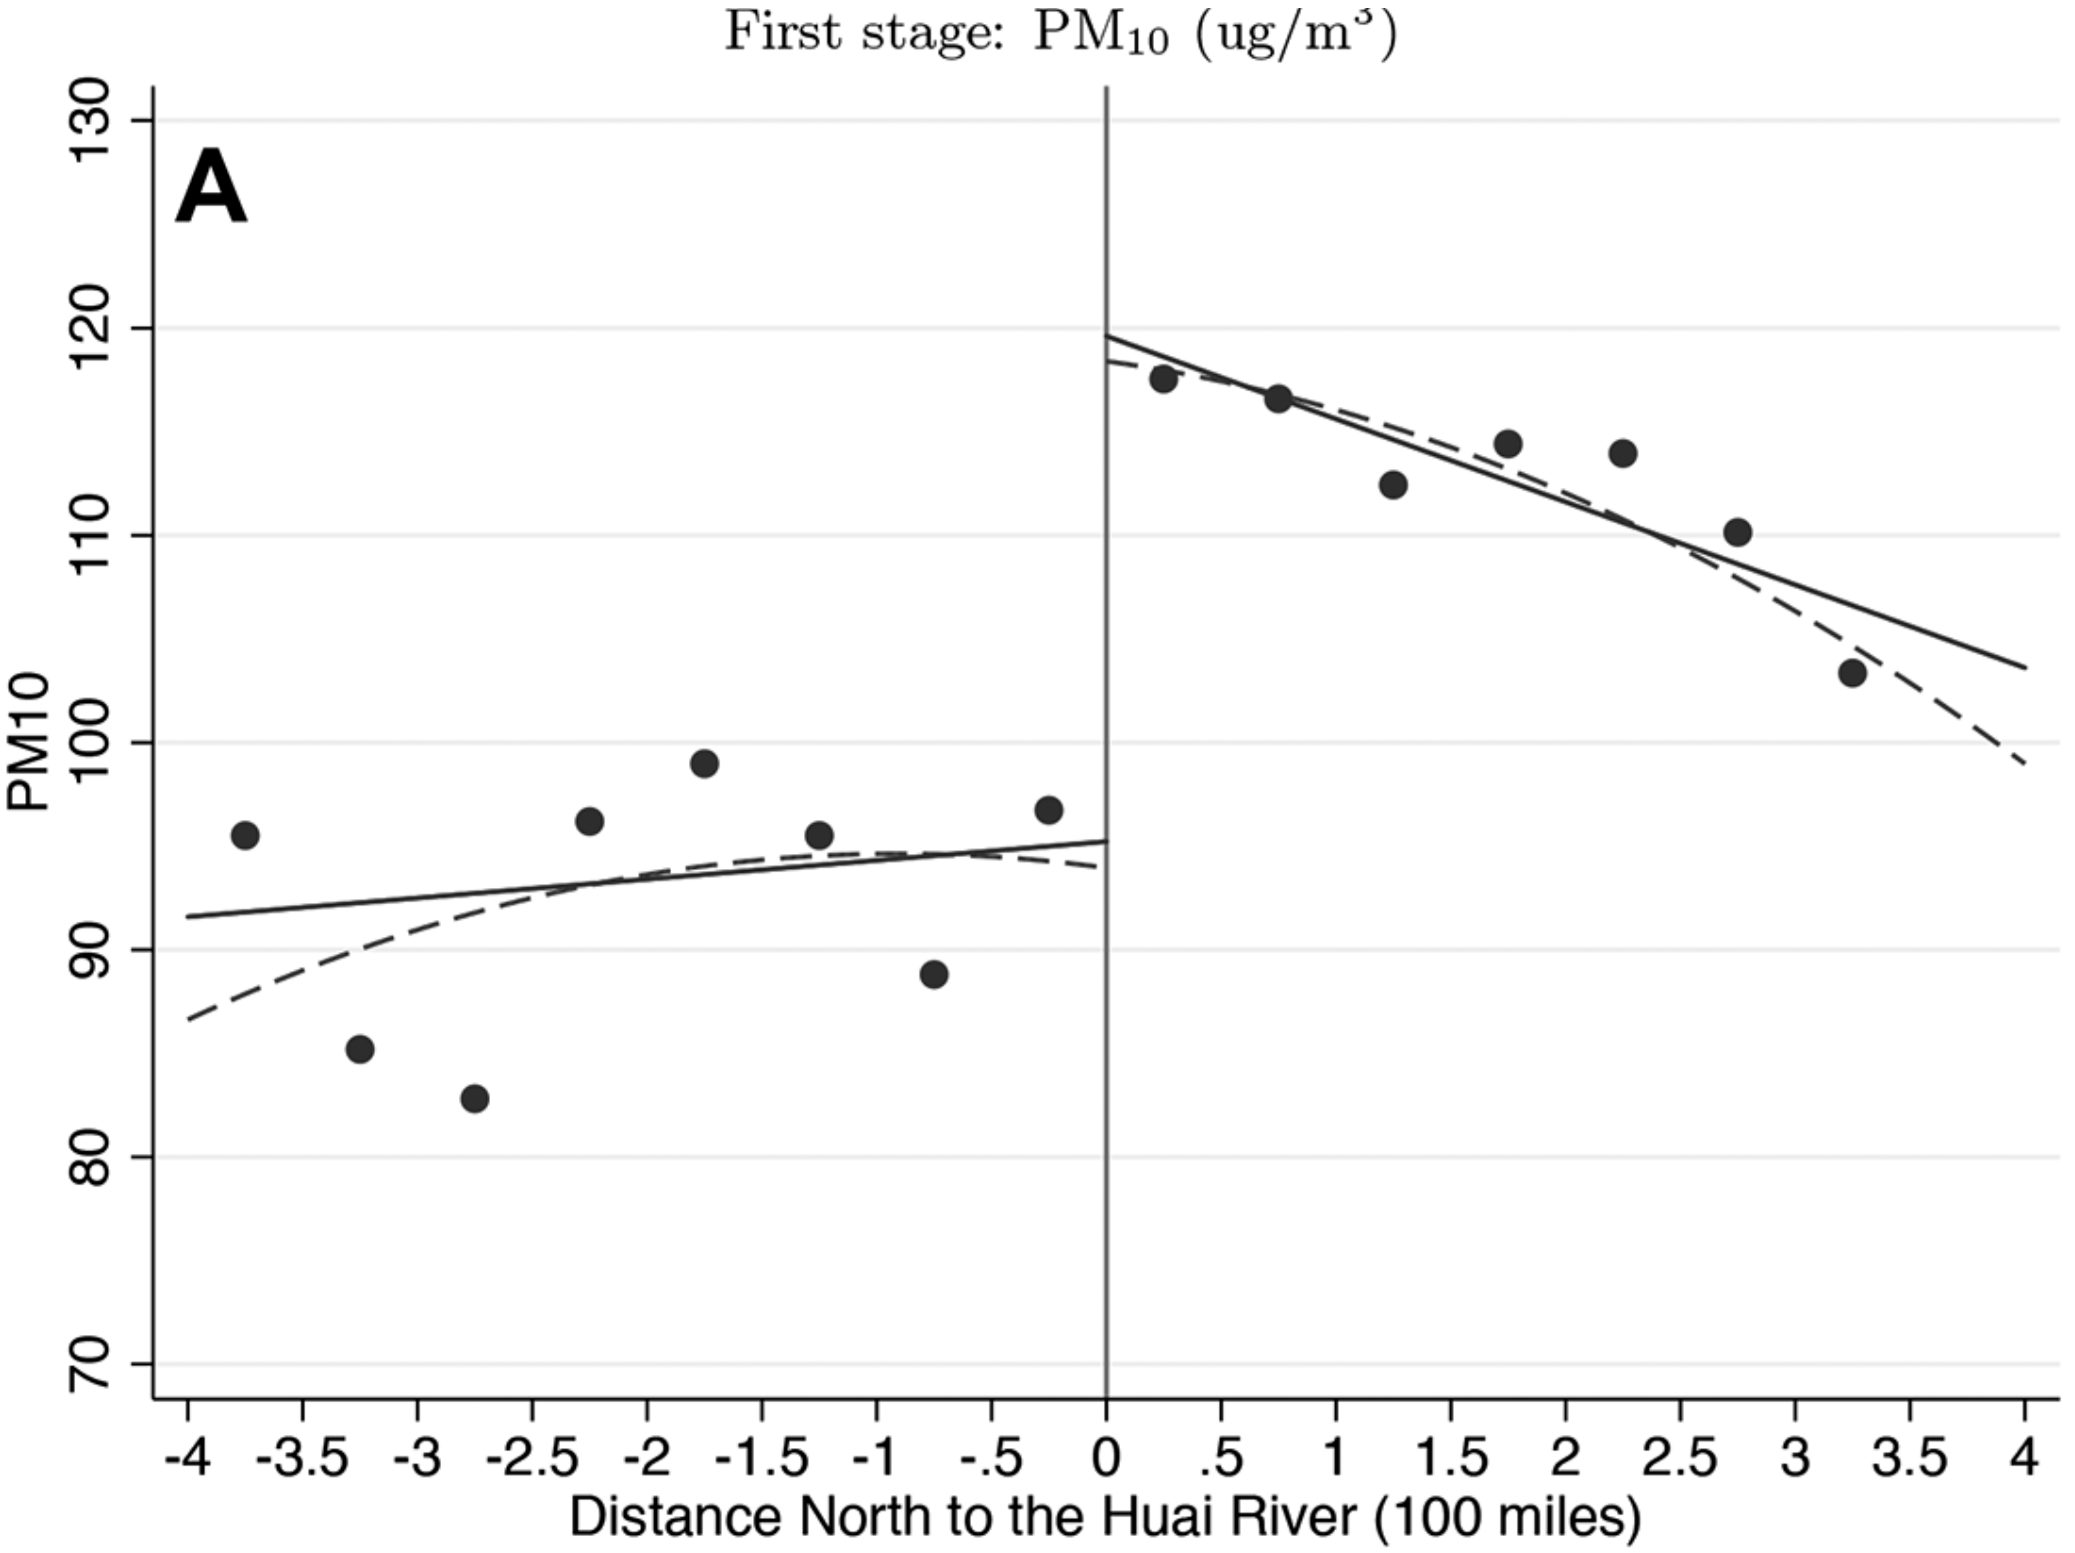
\includegraphics[scale=0.35]{figure2_1.png}
\end{frame}
%------------------------------------------------
\begin{frame}{B. Graphical Analysis of the RD Design}{RD at the Huai River boundary}
	\centering
	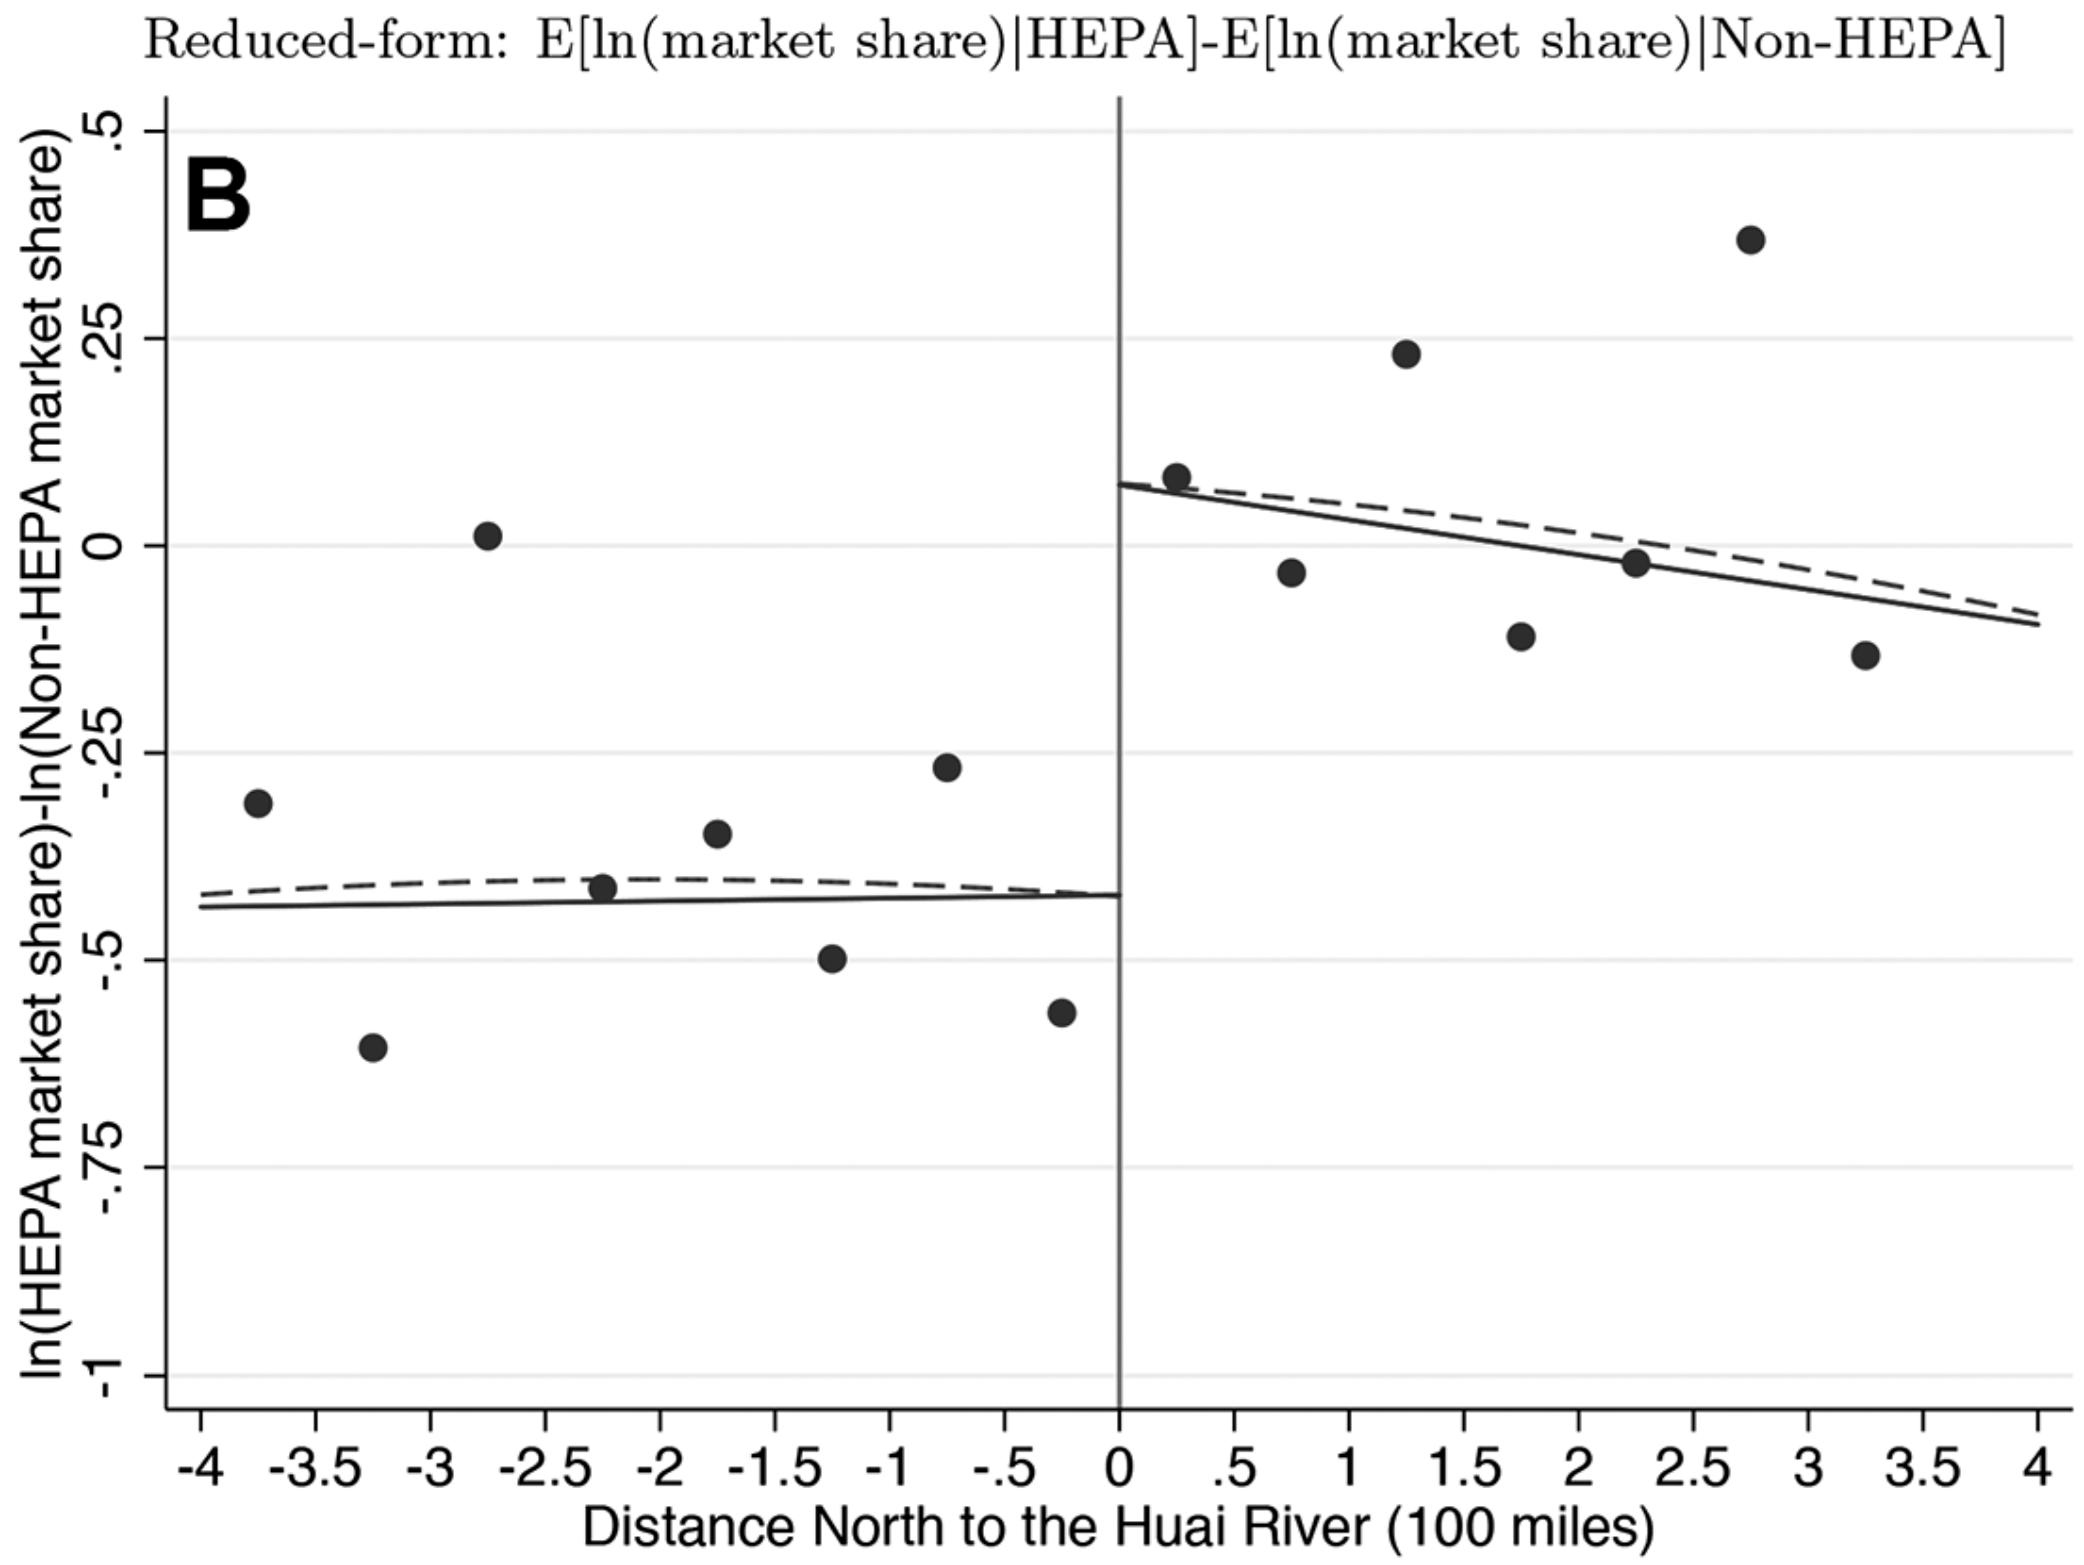
\includegraphics[scale=0.35]{figure2_2.png}
\end{frame}
%------------------------------------------------
\subsection{C. Baseline Results: Standard Logit Model}
\begin{frame}[shrink]
	\transfade
	\tableofcontents[sectionstyle=show/shaded,subsectionstyle=show/shaded/hide]
	\addtocounter{framenumber}{-1}
\end{frame}
%------------------------------------------------
\begin{frame}{C. Baseline Results: Standard Logit Model}
	\centering
	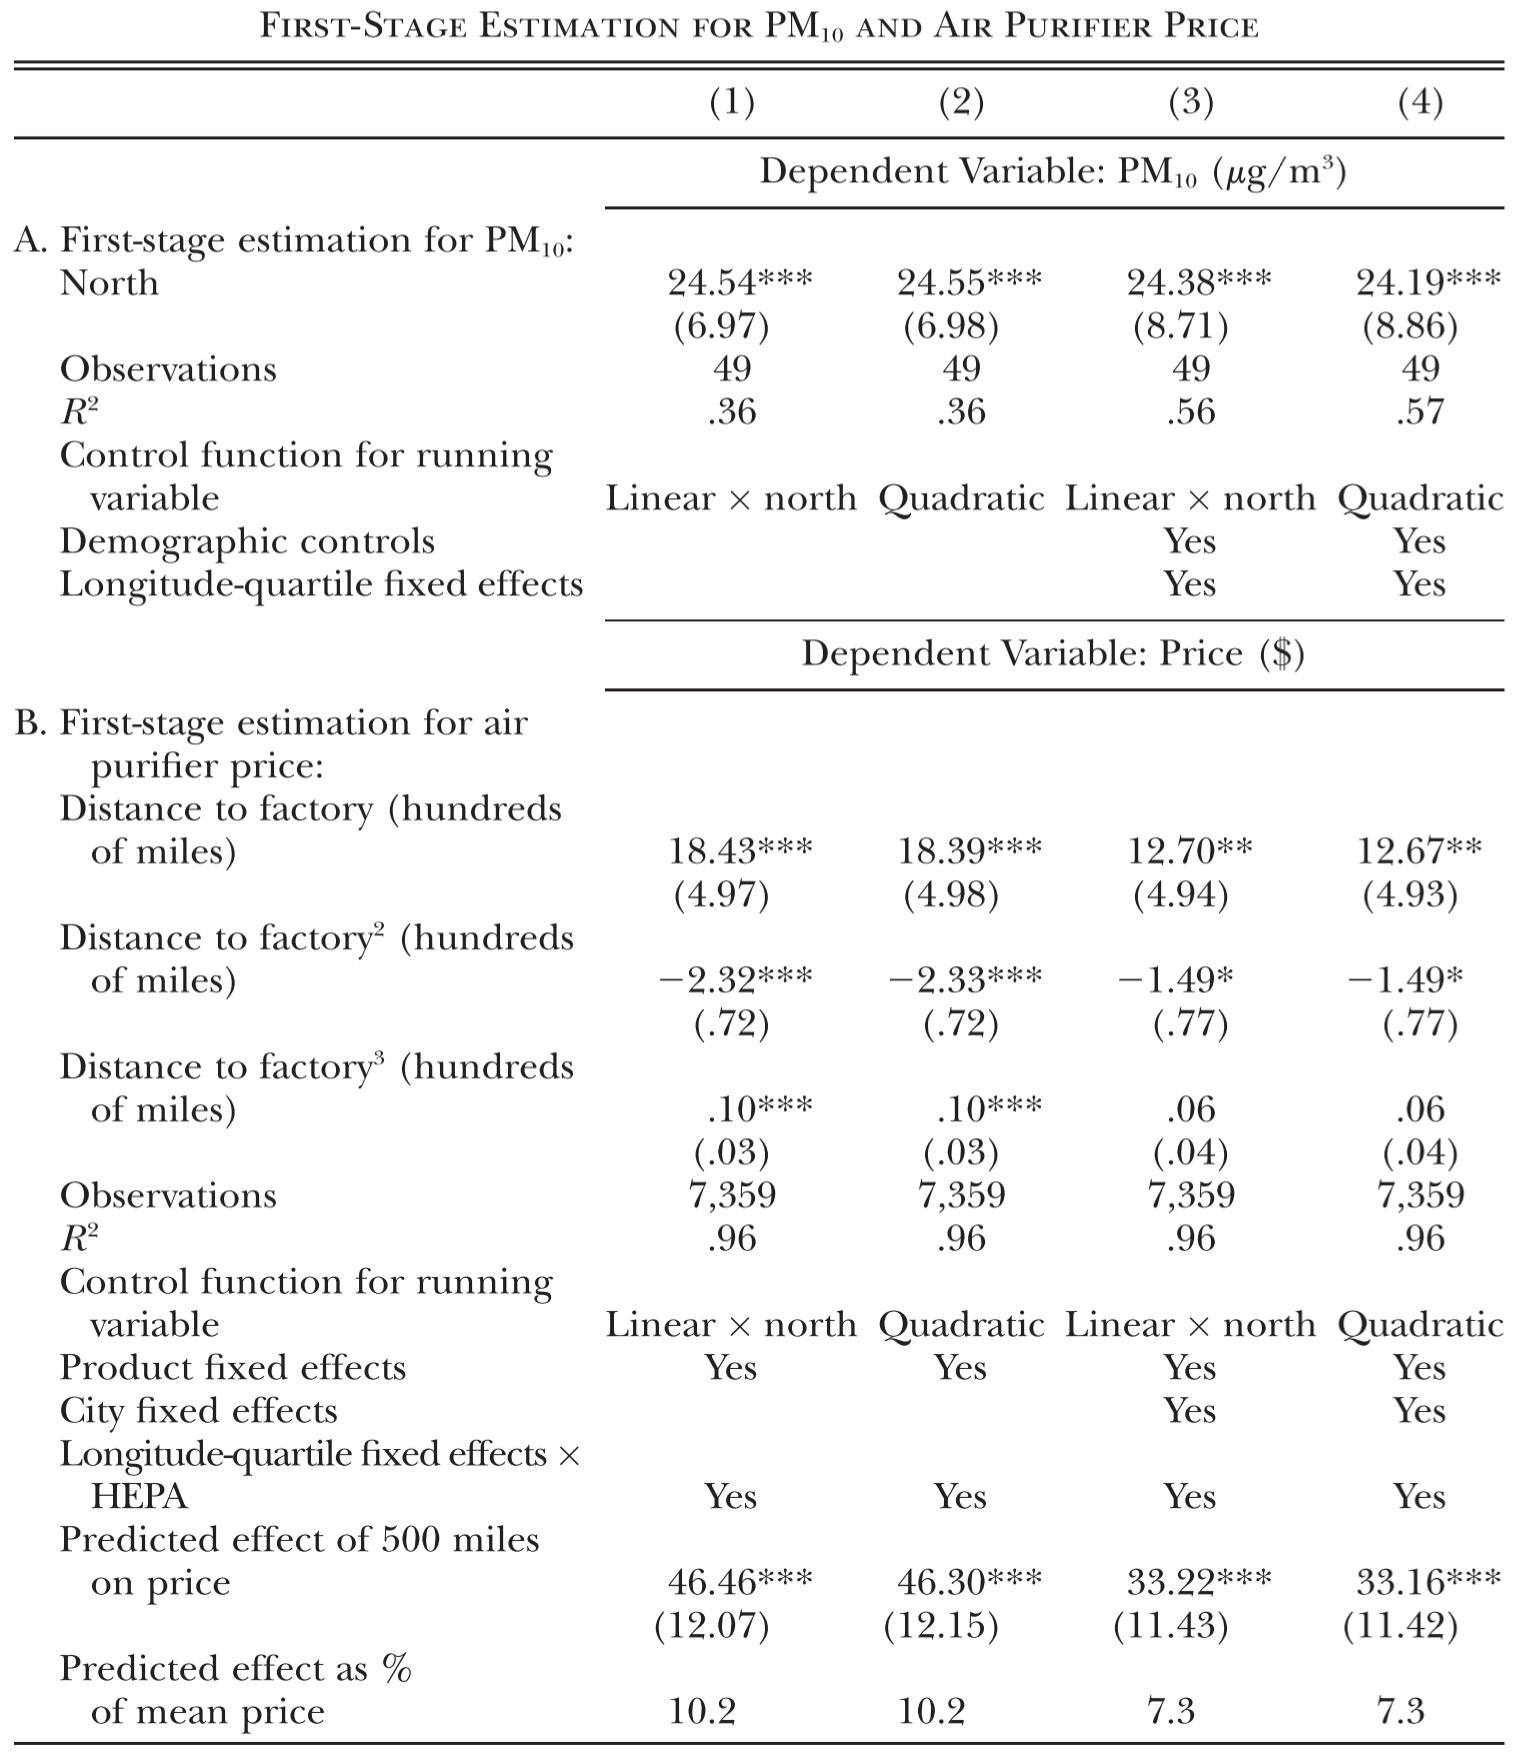
\includegraphics[scale=0.35]{table3.png}
\end{frame}
%------------------------------------------------
\begin{frame}{C. Baseline Results: Standard Logit Model}
	\centering
	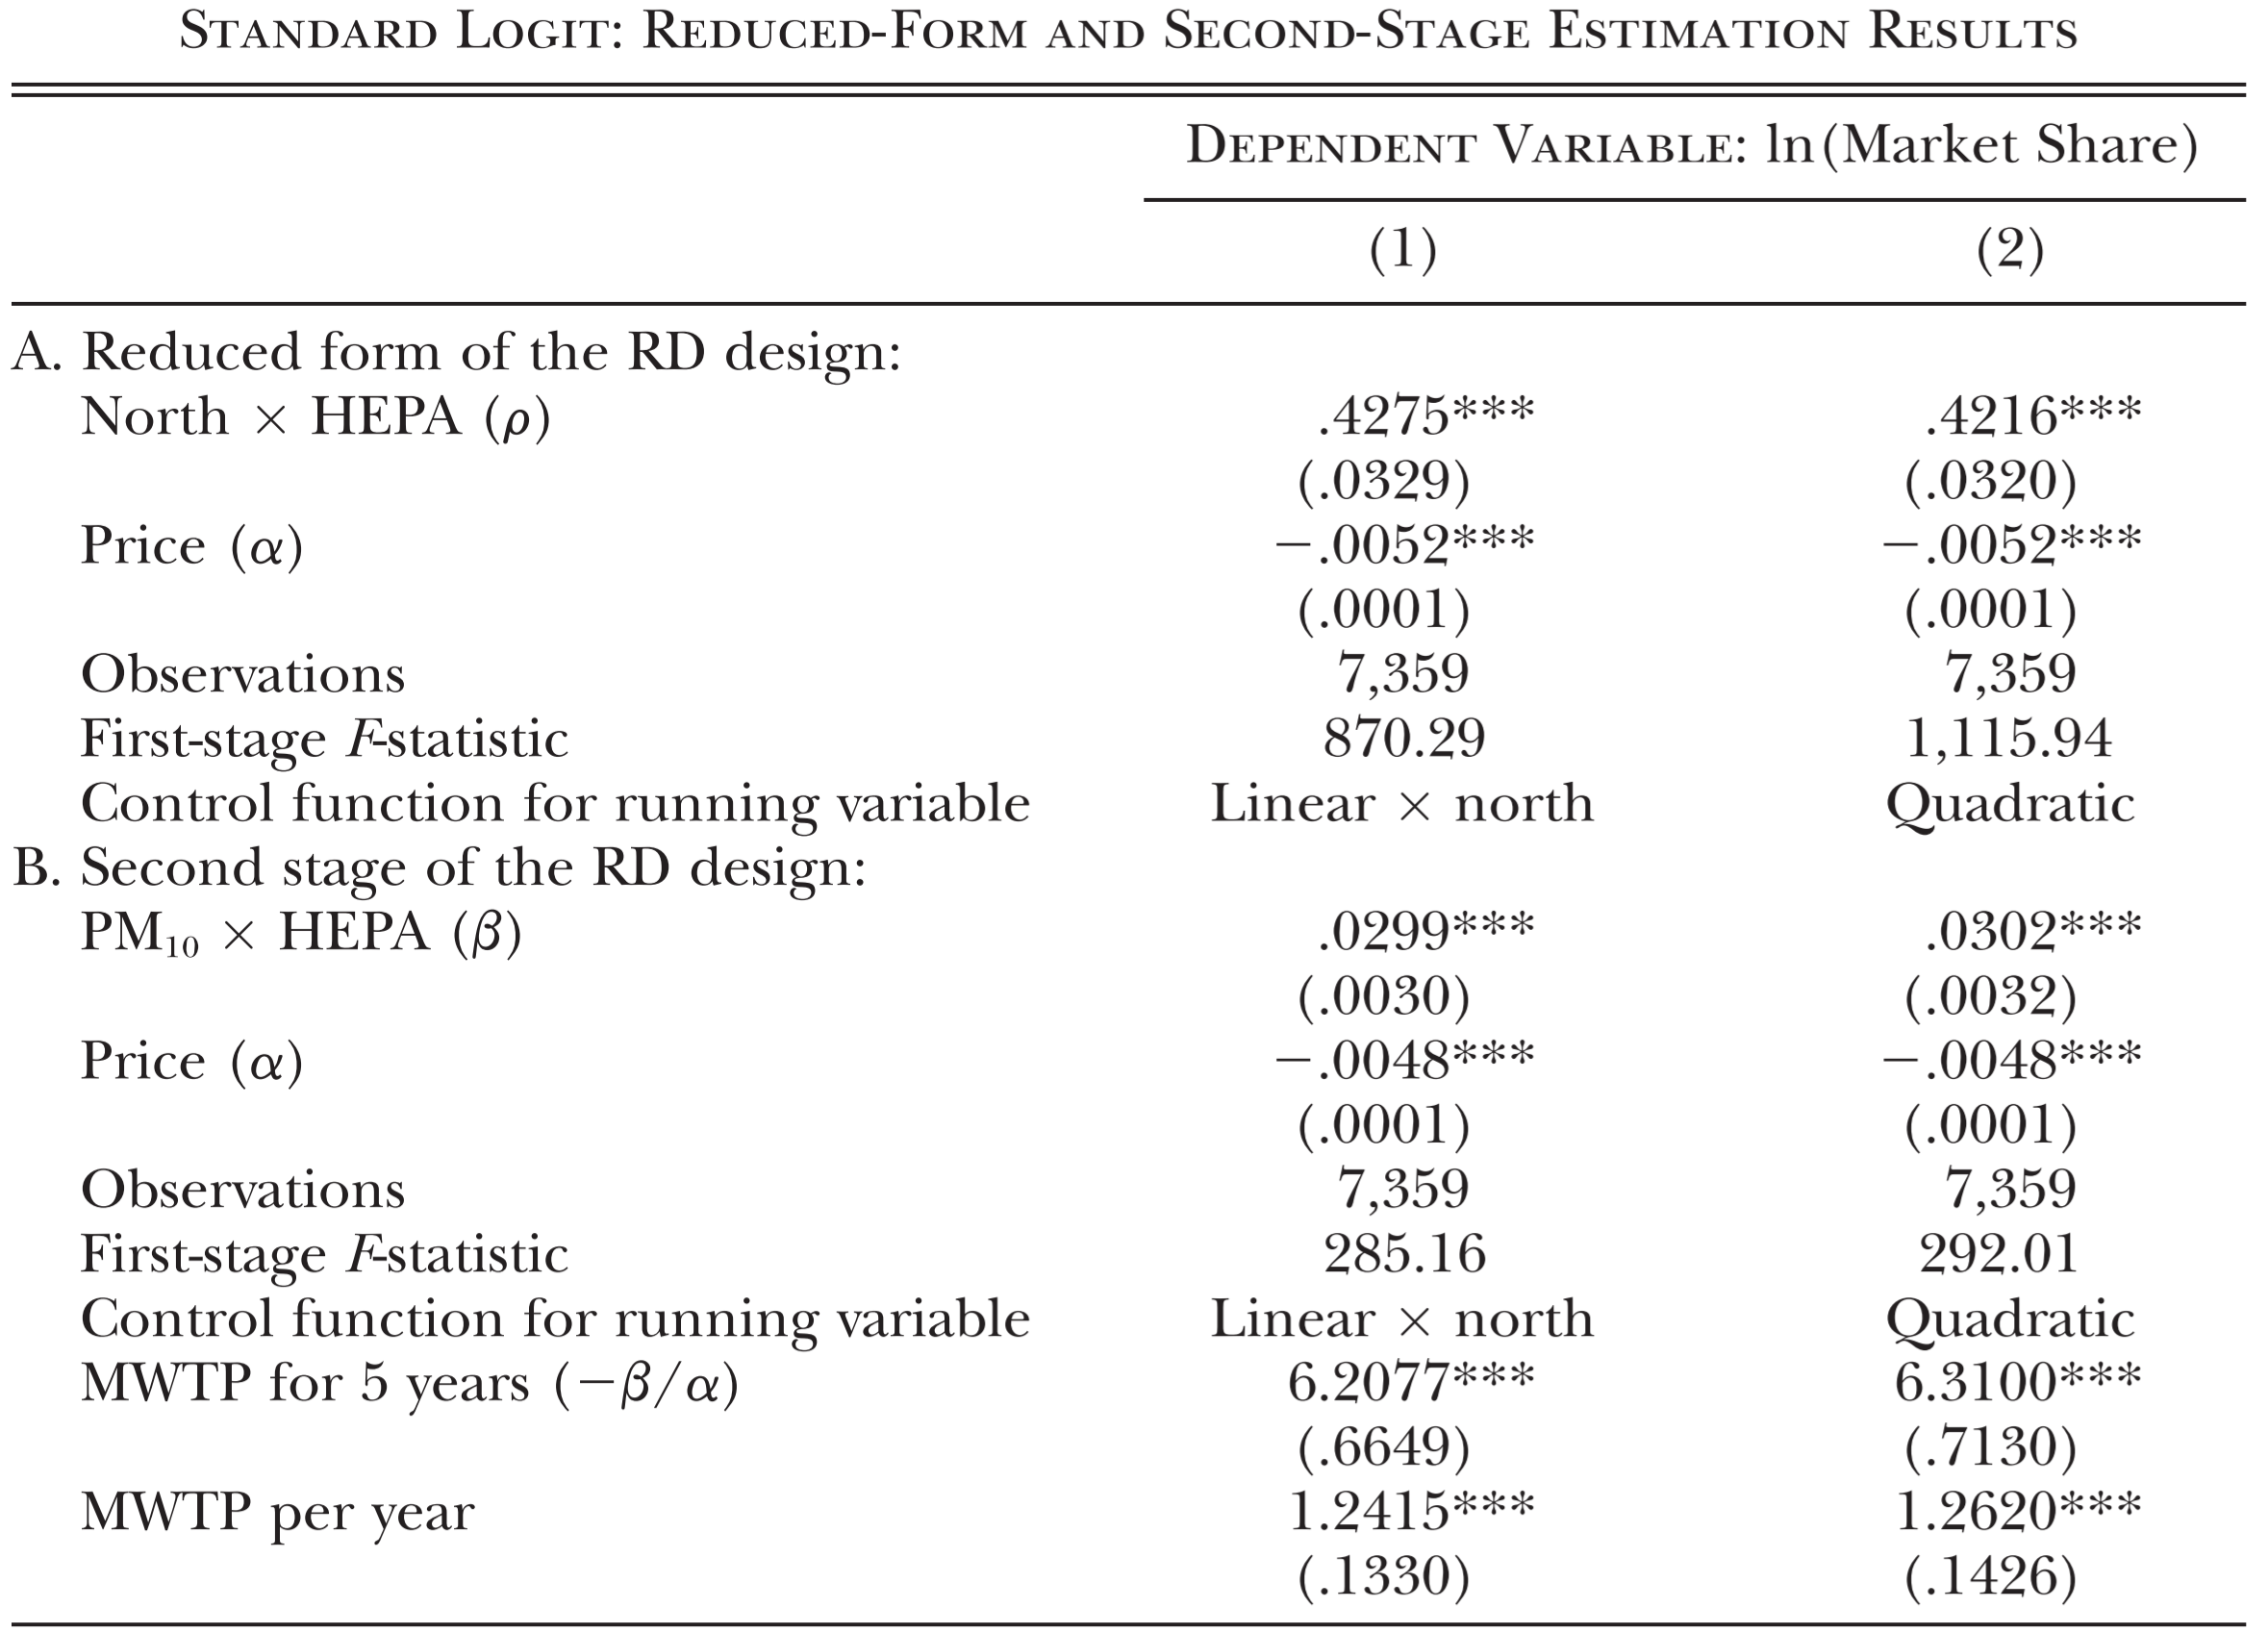
\includegraphics[scale=0.35]{table4.png}
\end{frame}
%------------------------------------------------
\begin{frame}{C. Baseline Results: Standard Logit Model}
	\centering
	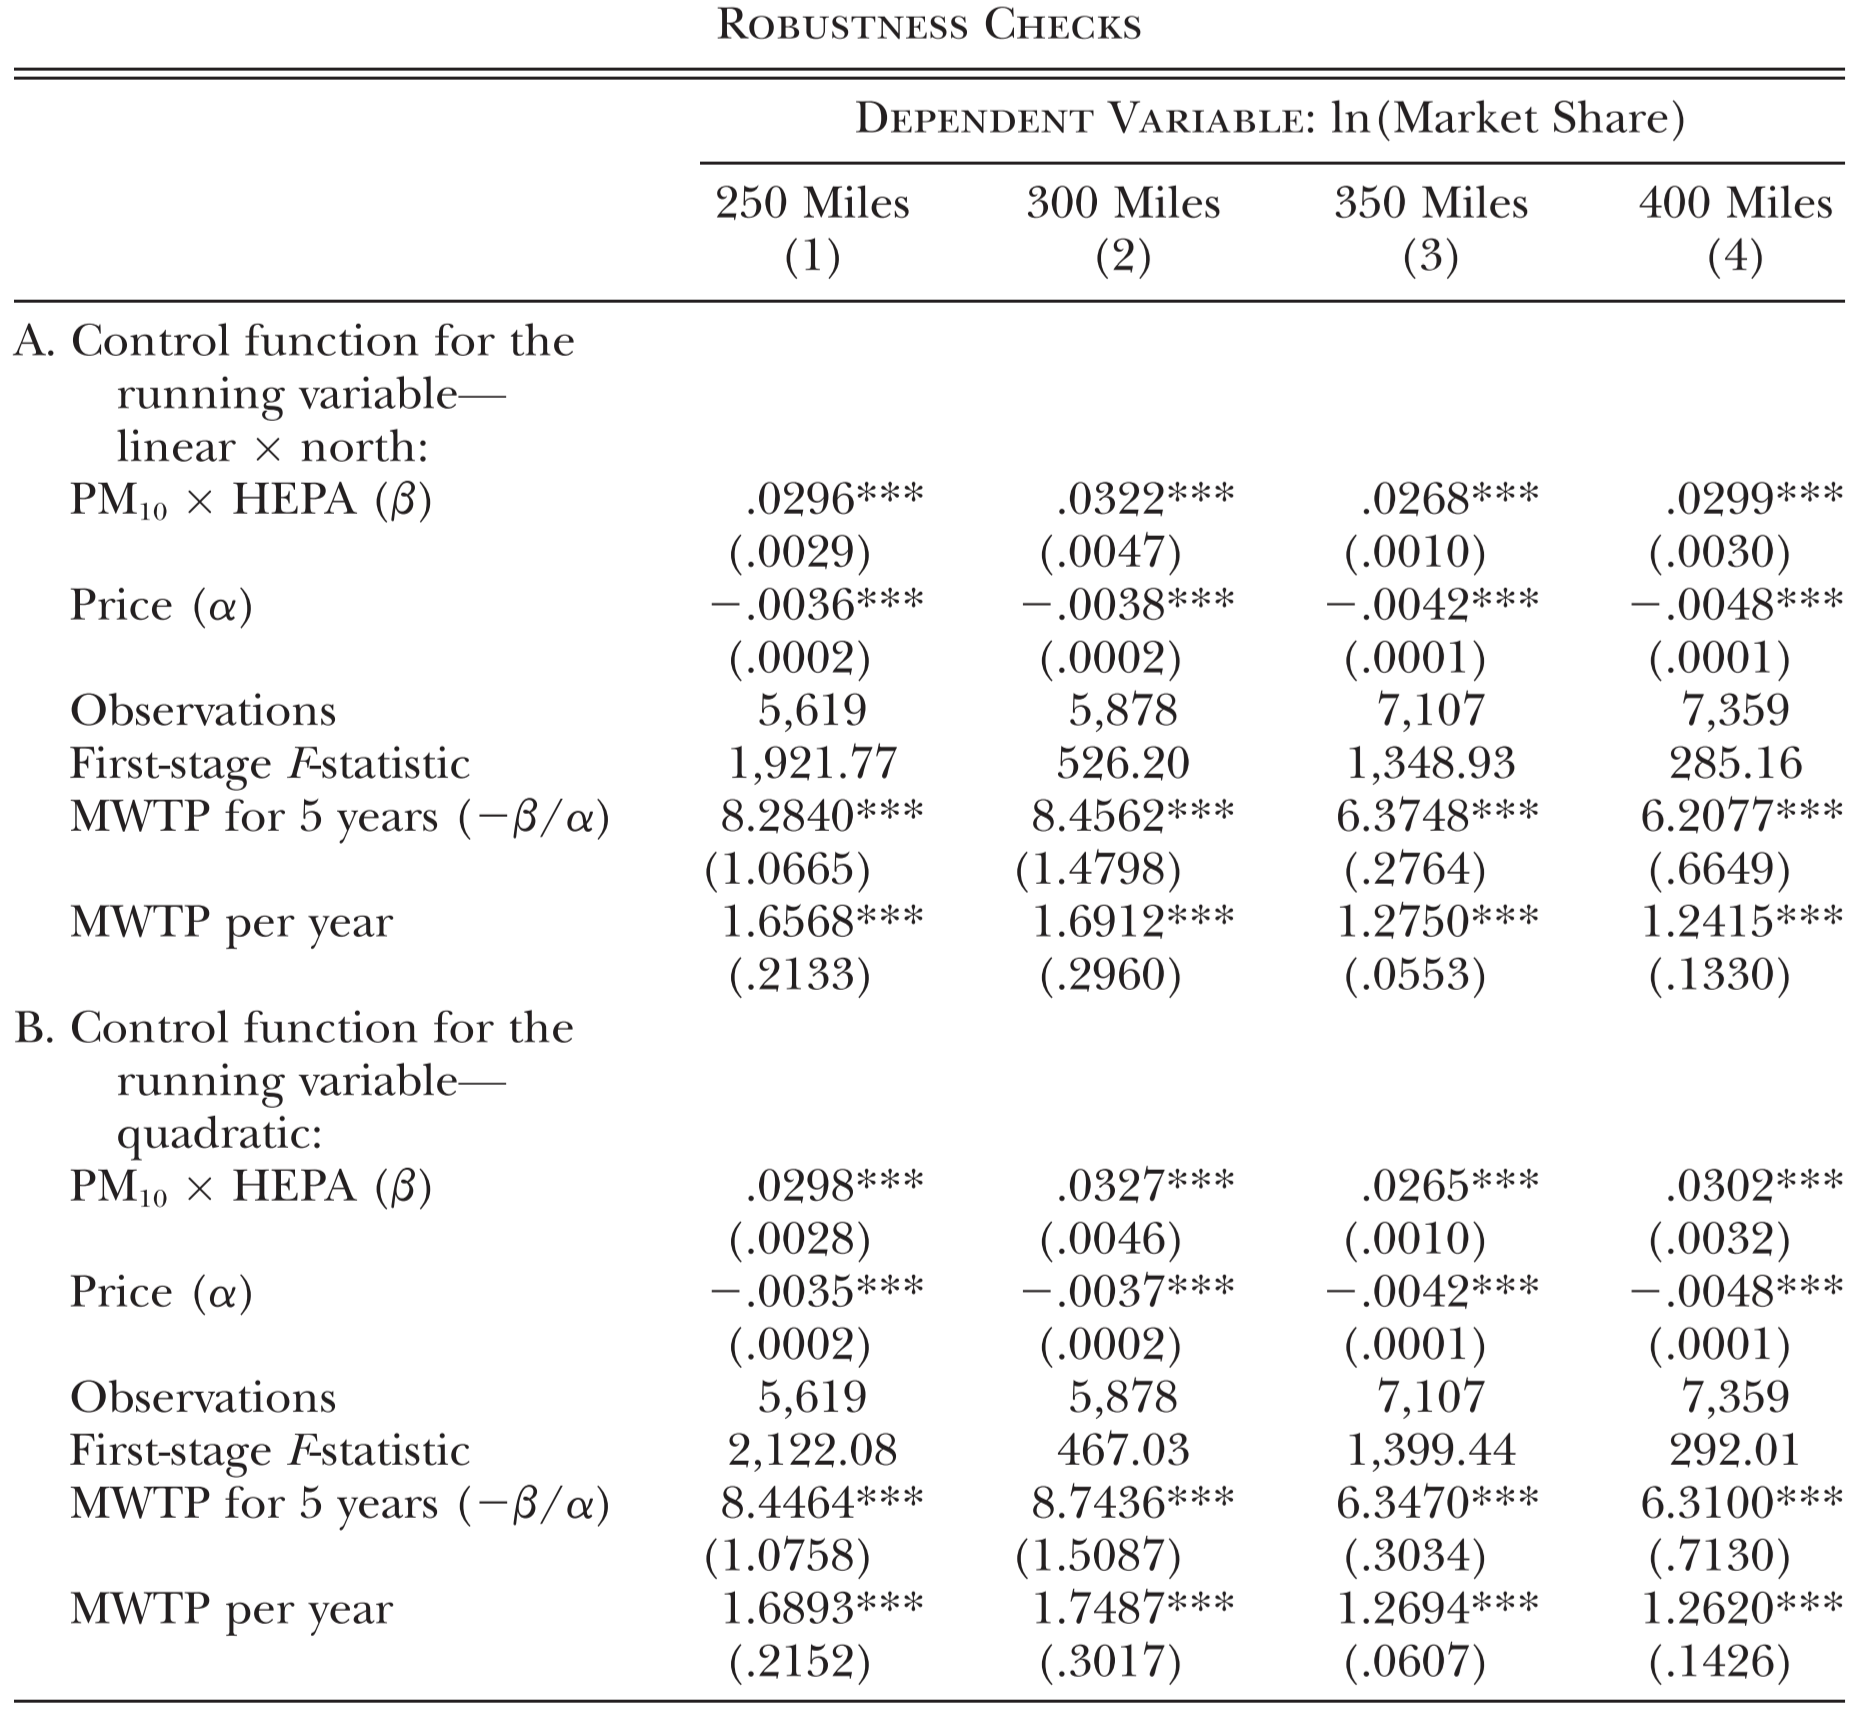
\includegraphics[scale=0.35]{table5.png}
\end{frame}
%------------------------------------------------
\subsection{D. Role of Information in WTP for Clean Air}
\begin{frame}[shrink]
	\transfade
	\tableofcontents[sectionstyle=show/shaded,subsectionstyle=show/shaded/hide]
	\addtocounter{framenumber}{-1}
\end{frame}
%------------------------------------------------
\begin{frame}{D. Role of Information in WTP for Clean Air}
	\centering
	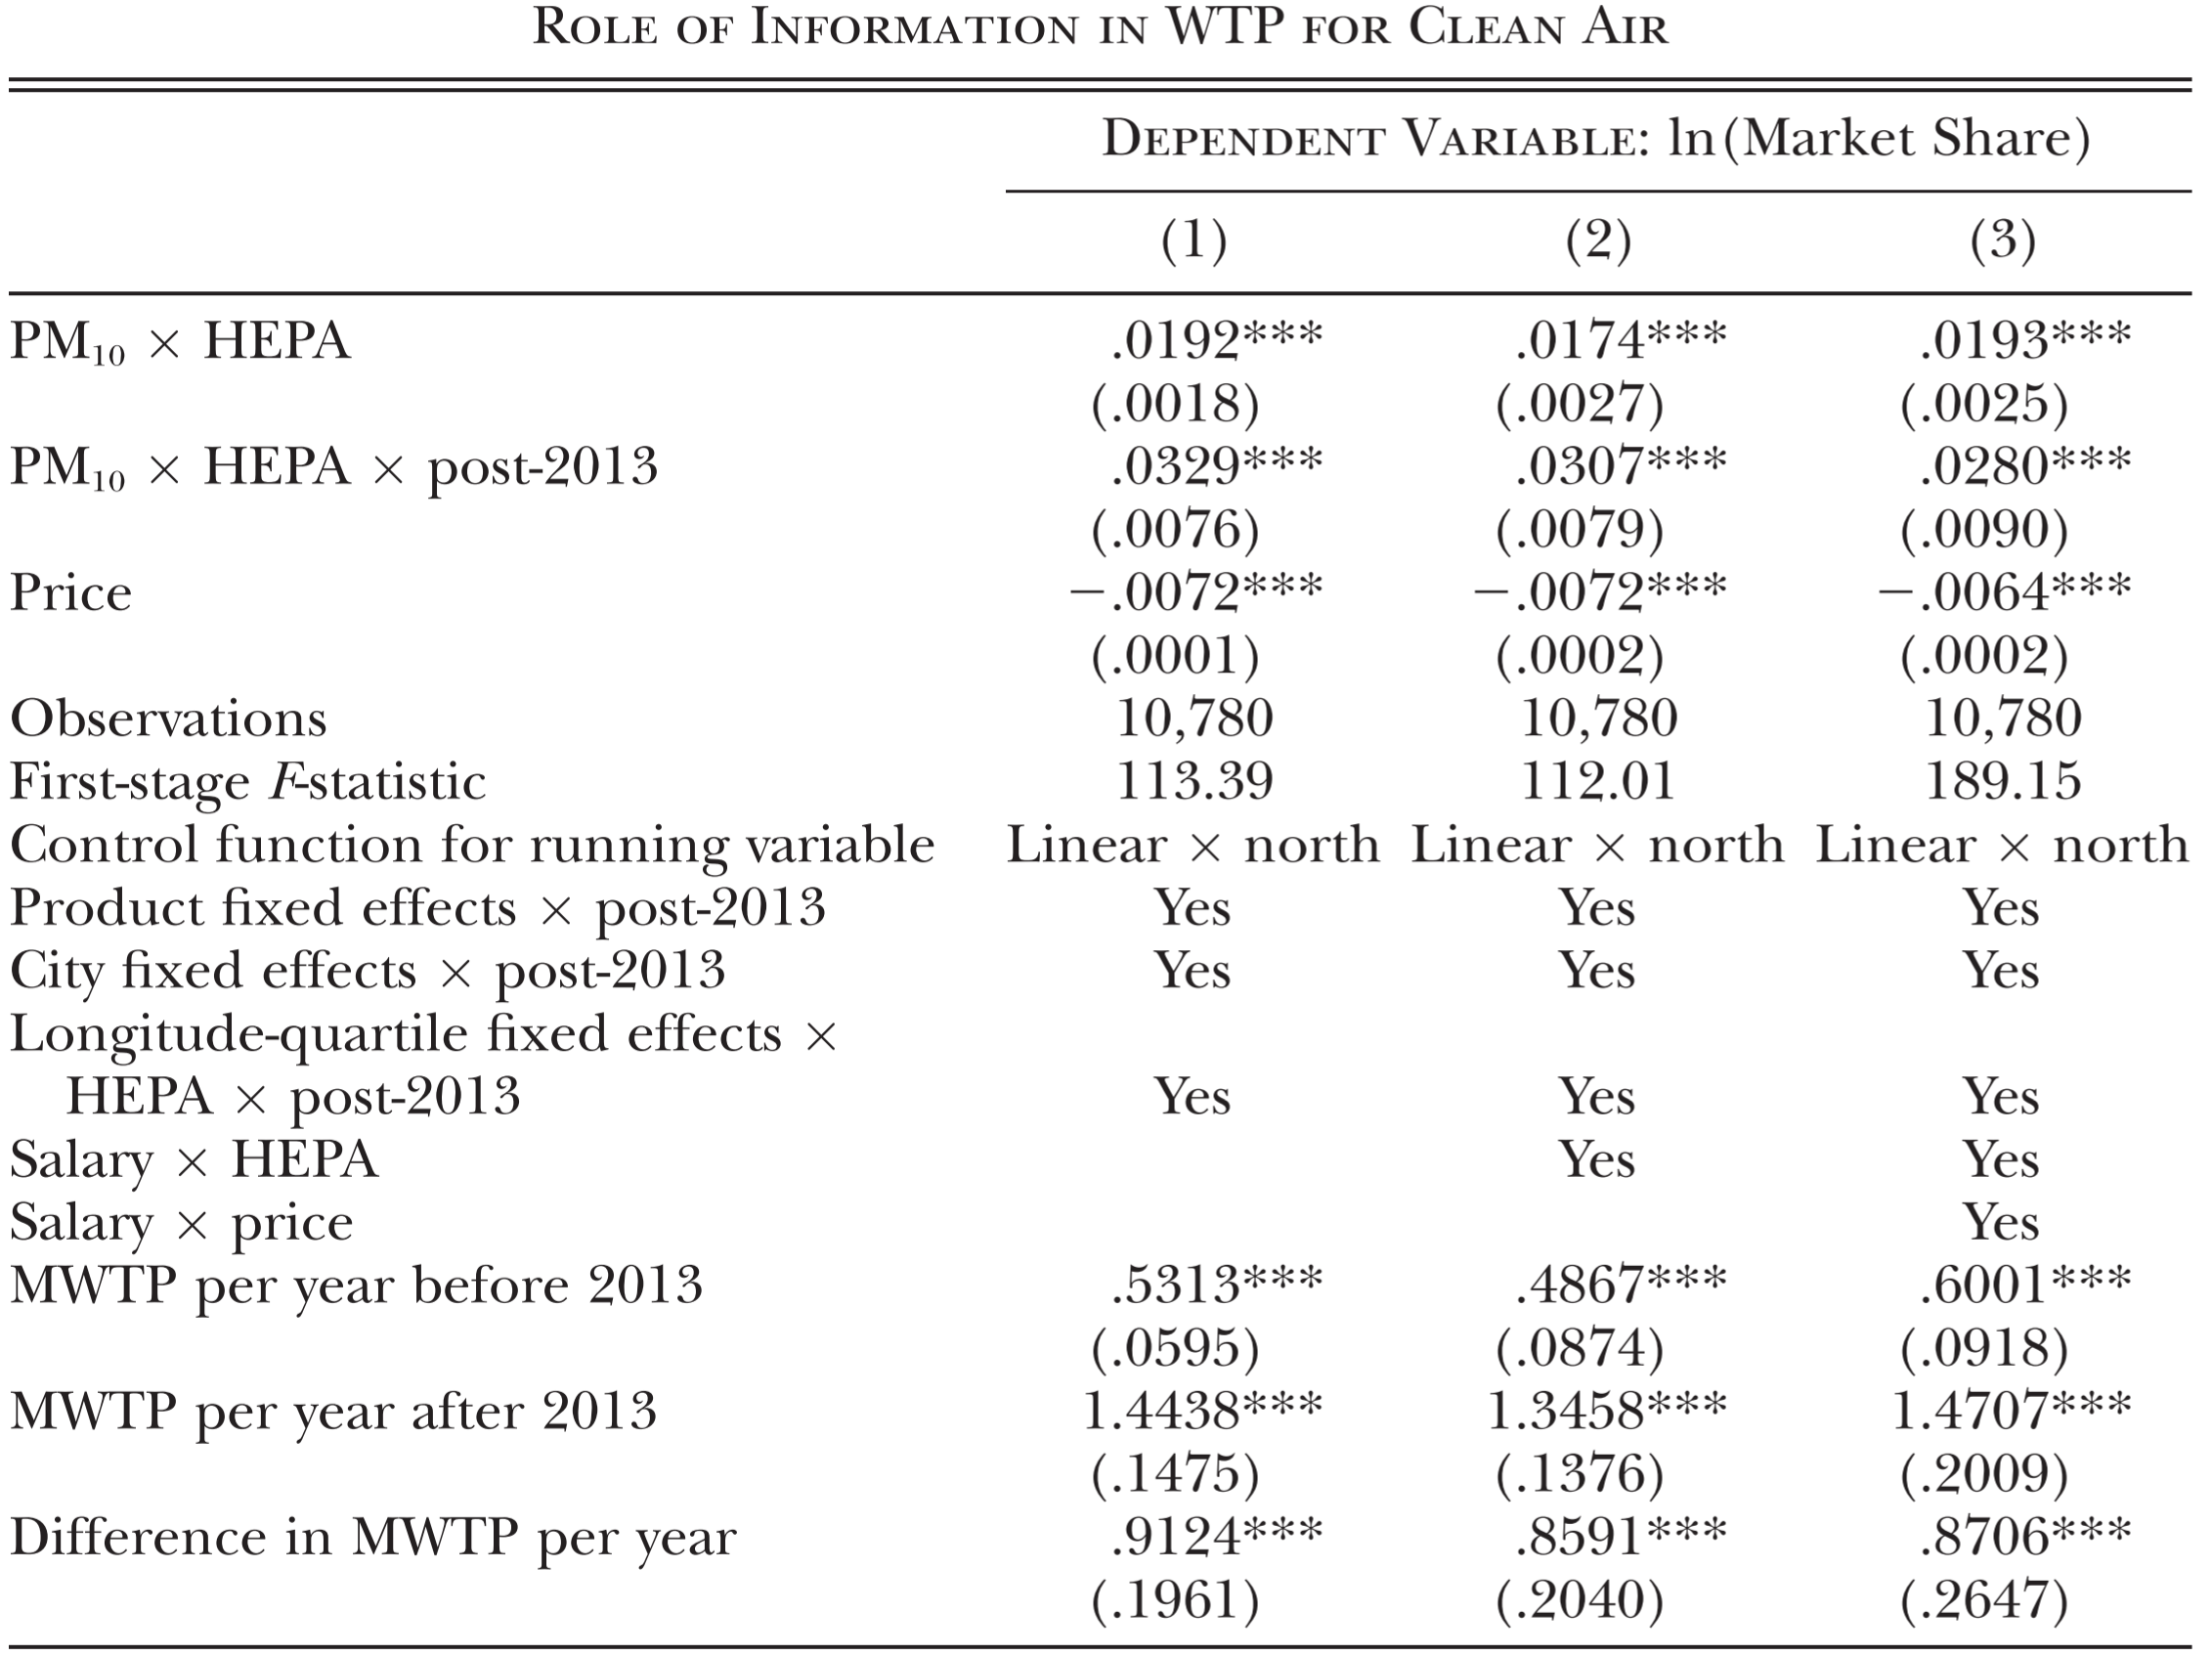
\includegraphics[scale=0.35]{table6.png}	
\end{frame}
%------------------------------------------------
\subsection{E. Heterogeneity in WTP for Clean Air}
\begin{frame}[shrink]
	\transfade %fade in and fade out
	\tableofcontents[sectionstyle=show/shaded,subsectionstyle=show/shaded/hide]
	\addtocounter{framenumber}{-1}
\end{frame}
%------------------------------------------------
\begin{frame}{E. Heterogeneity in WTP for Clean Air}
	\centering
	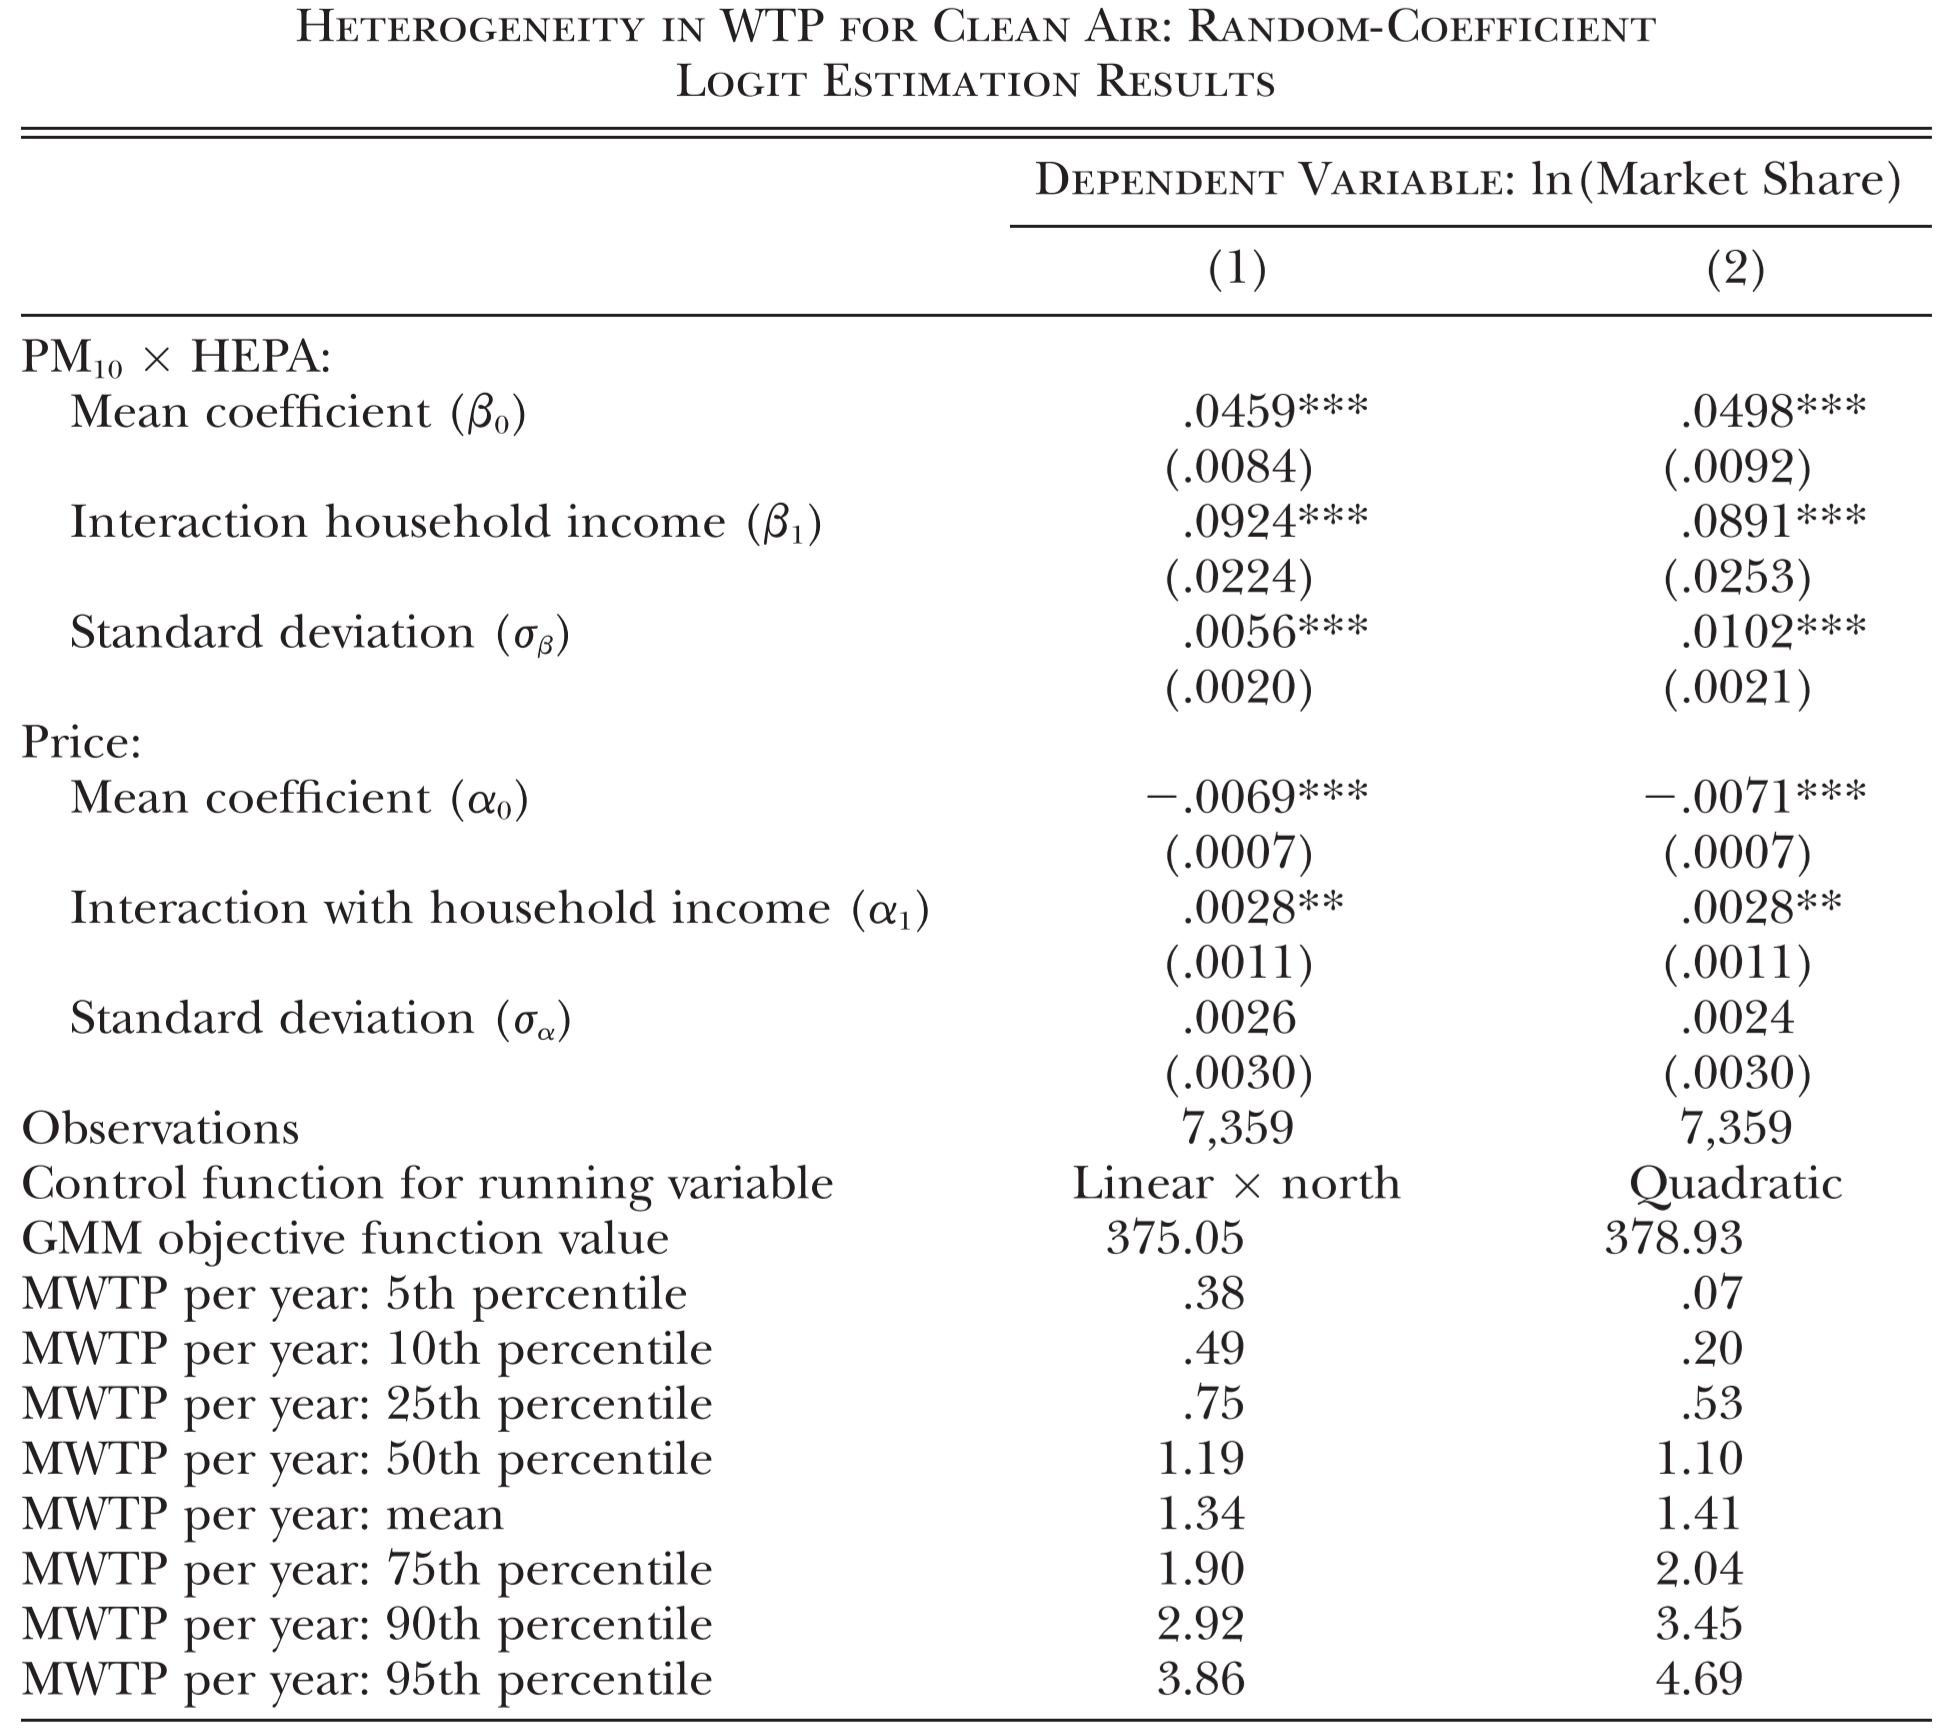
\includegraphics[scale=0.35]{table7.png}	
\end{frame}
%------------------------------------------------
\begin{frame}{E. Heterogeneity in WTP for Clean Air}
	\centering
	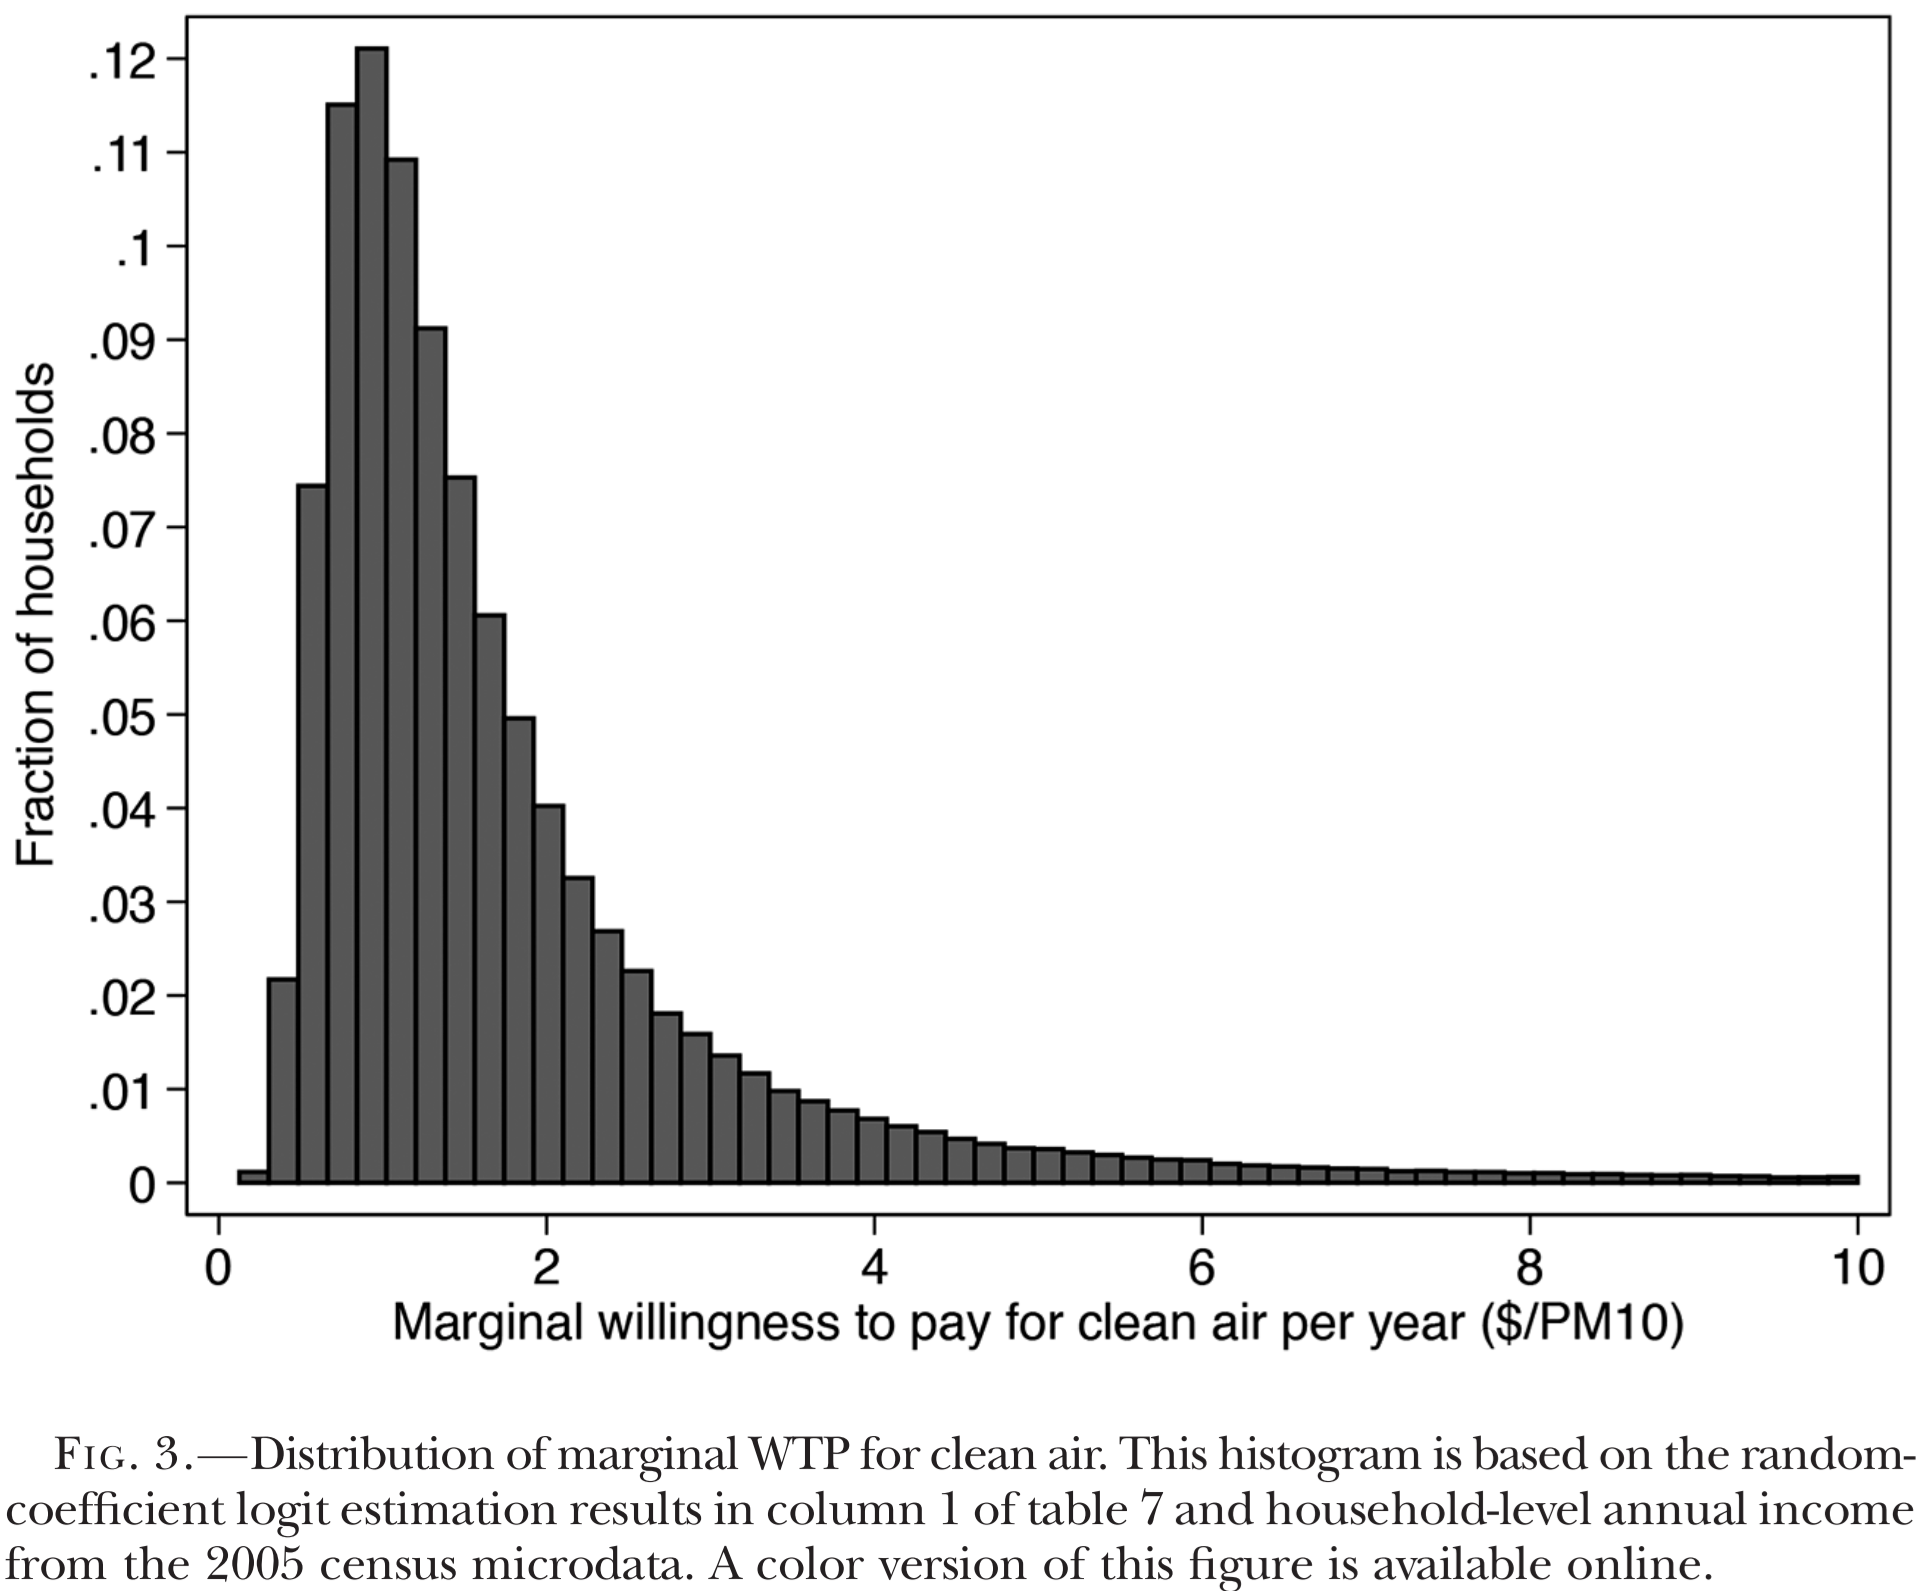
\includegraphics[scale=0.37]{figure3.png}	
\end{frame}
%------------------------------------------------
\begin{frame}{E. Heterogeneity in WTP for Clean Air}
	\centering
	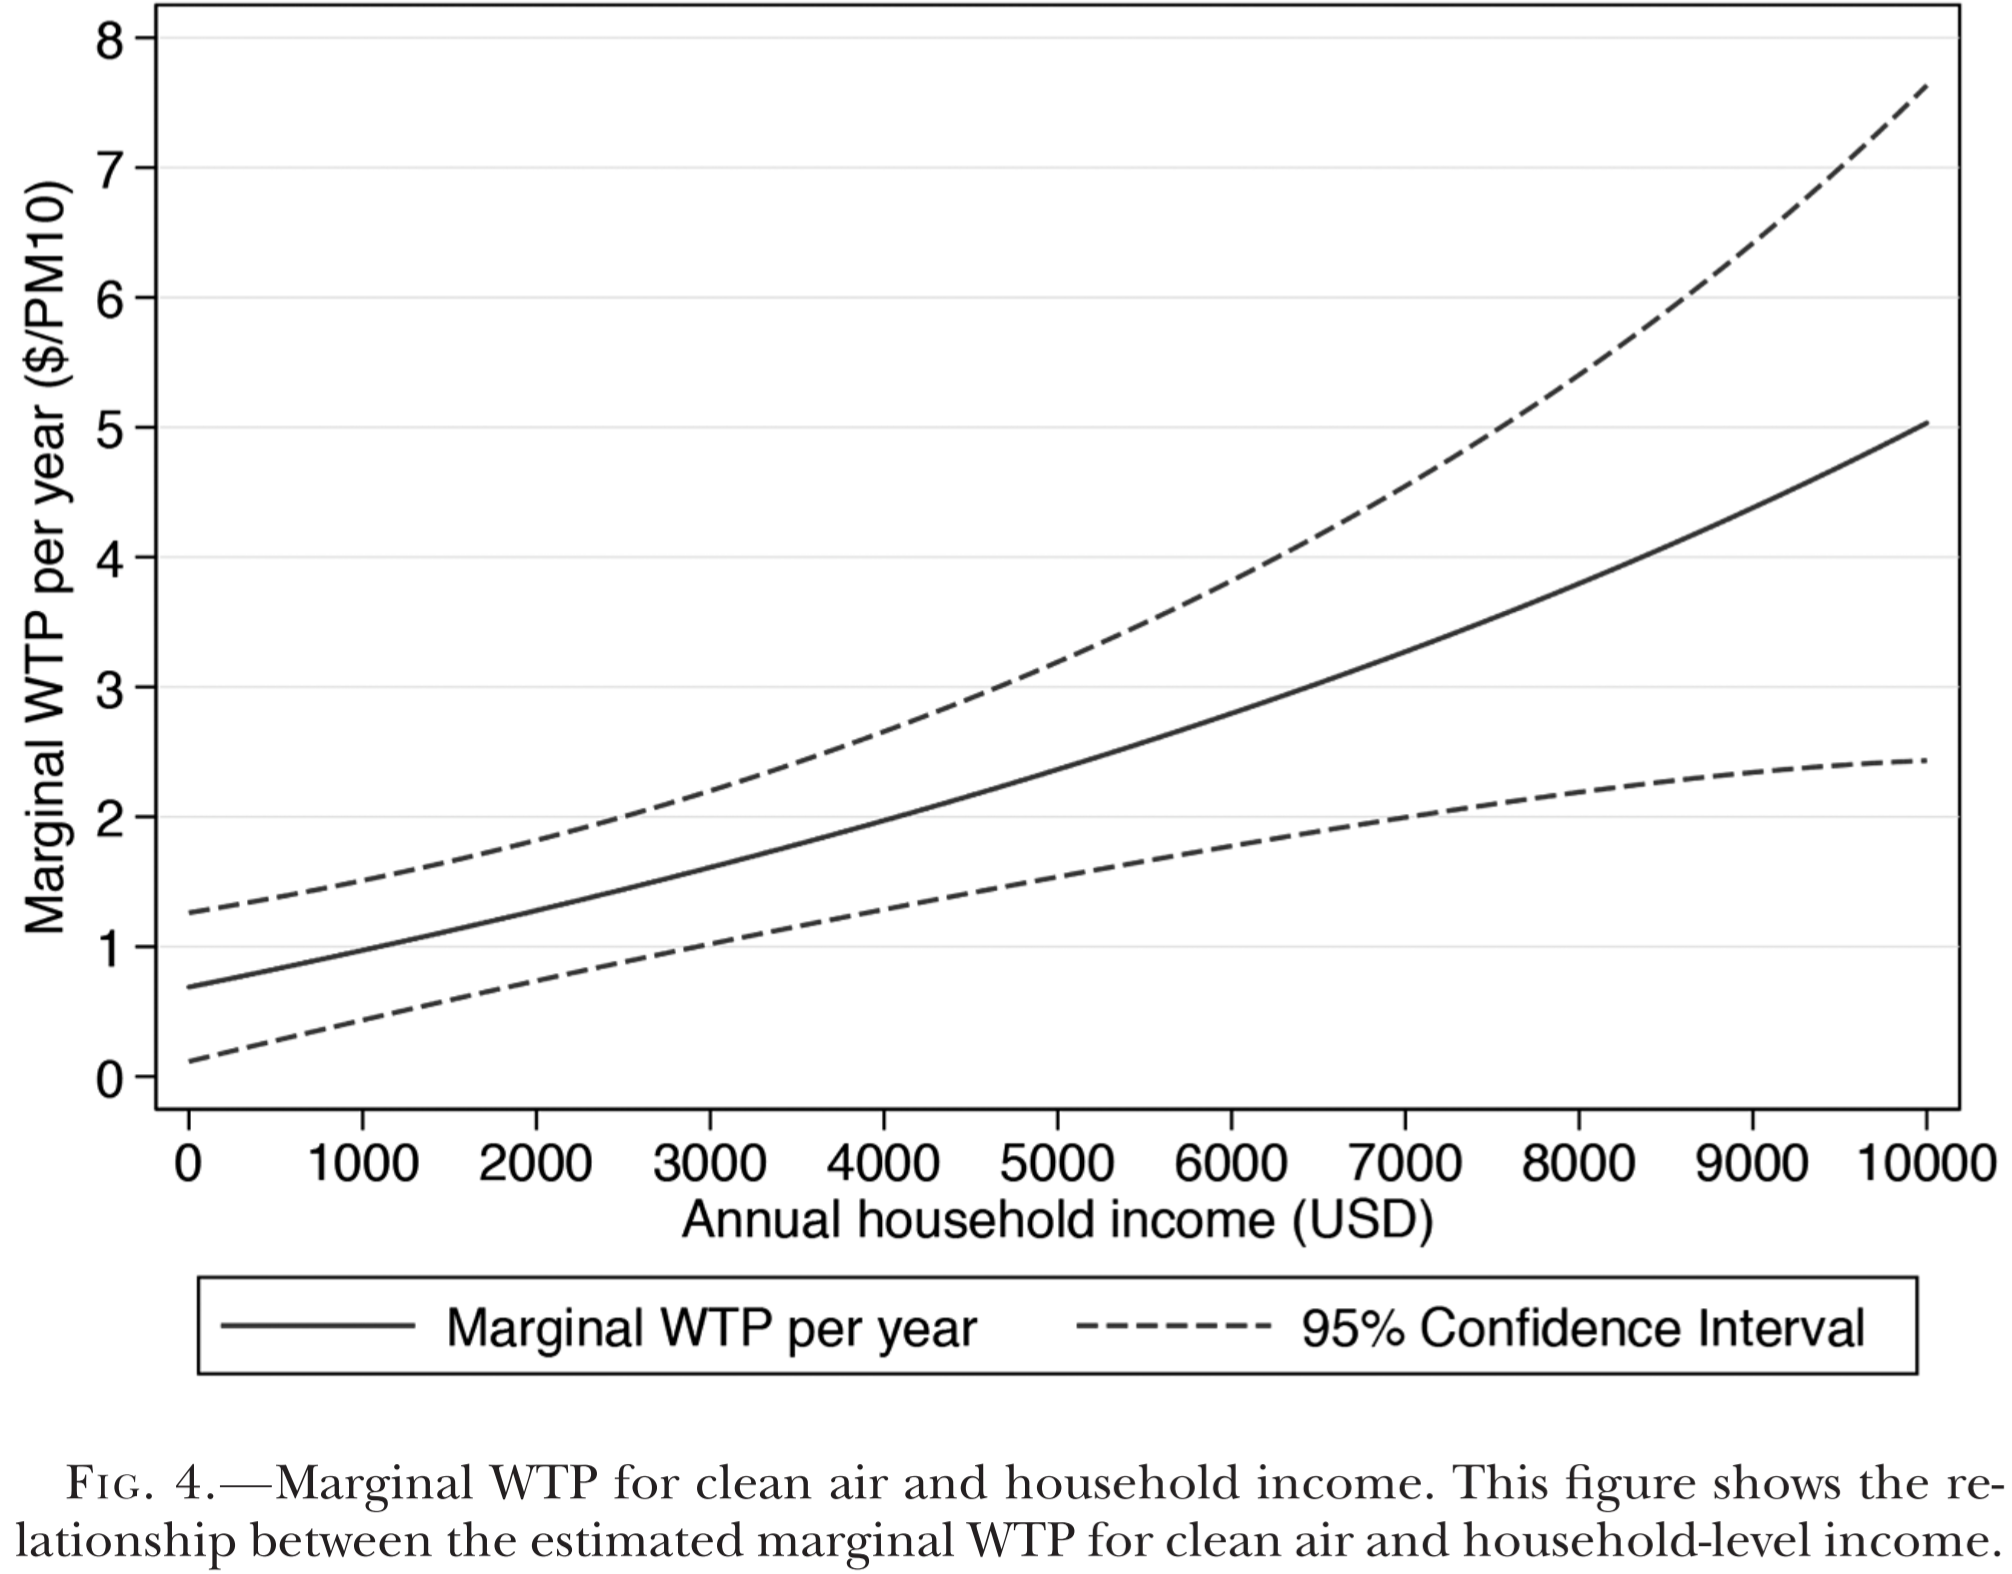
\includegraphics[scale=0.37]{figure4.png}	
\end{frame}
%------------------------------------------------

%------------------------------------------------
\section{Policy Implications}
\begin{frame}[shrink]
	\transfade %fade in and fade out
	\tableofcontents[sectionstyle=show/shaded,subsectionstyle=show/shaded/hide]
	\addtocounter{framenumber}{-1}
\end{frame}
%------------------------------------------------
\begin{frame}{E. Heterogeneity in WTP for Clean Air}
	\centering
	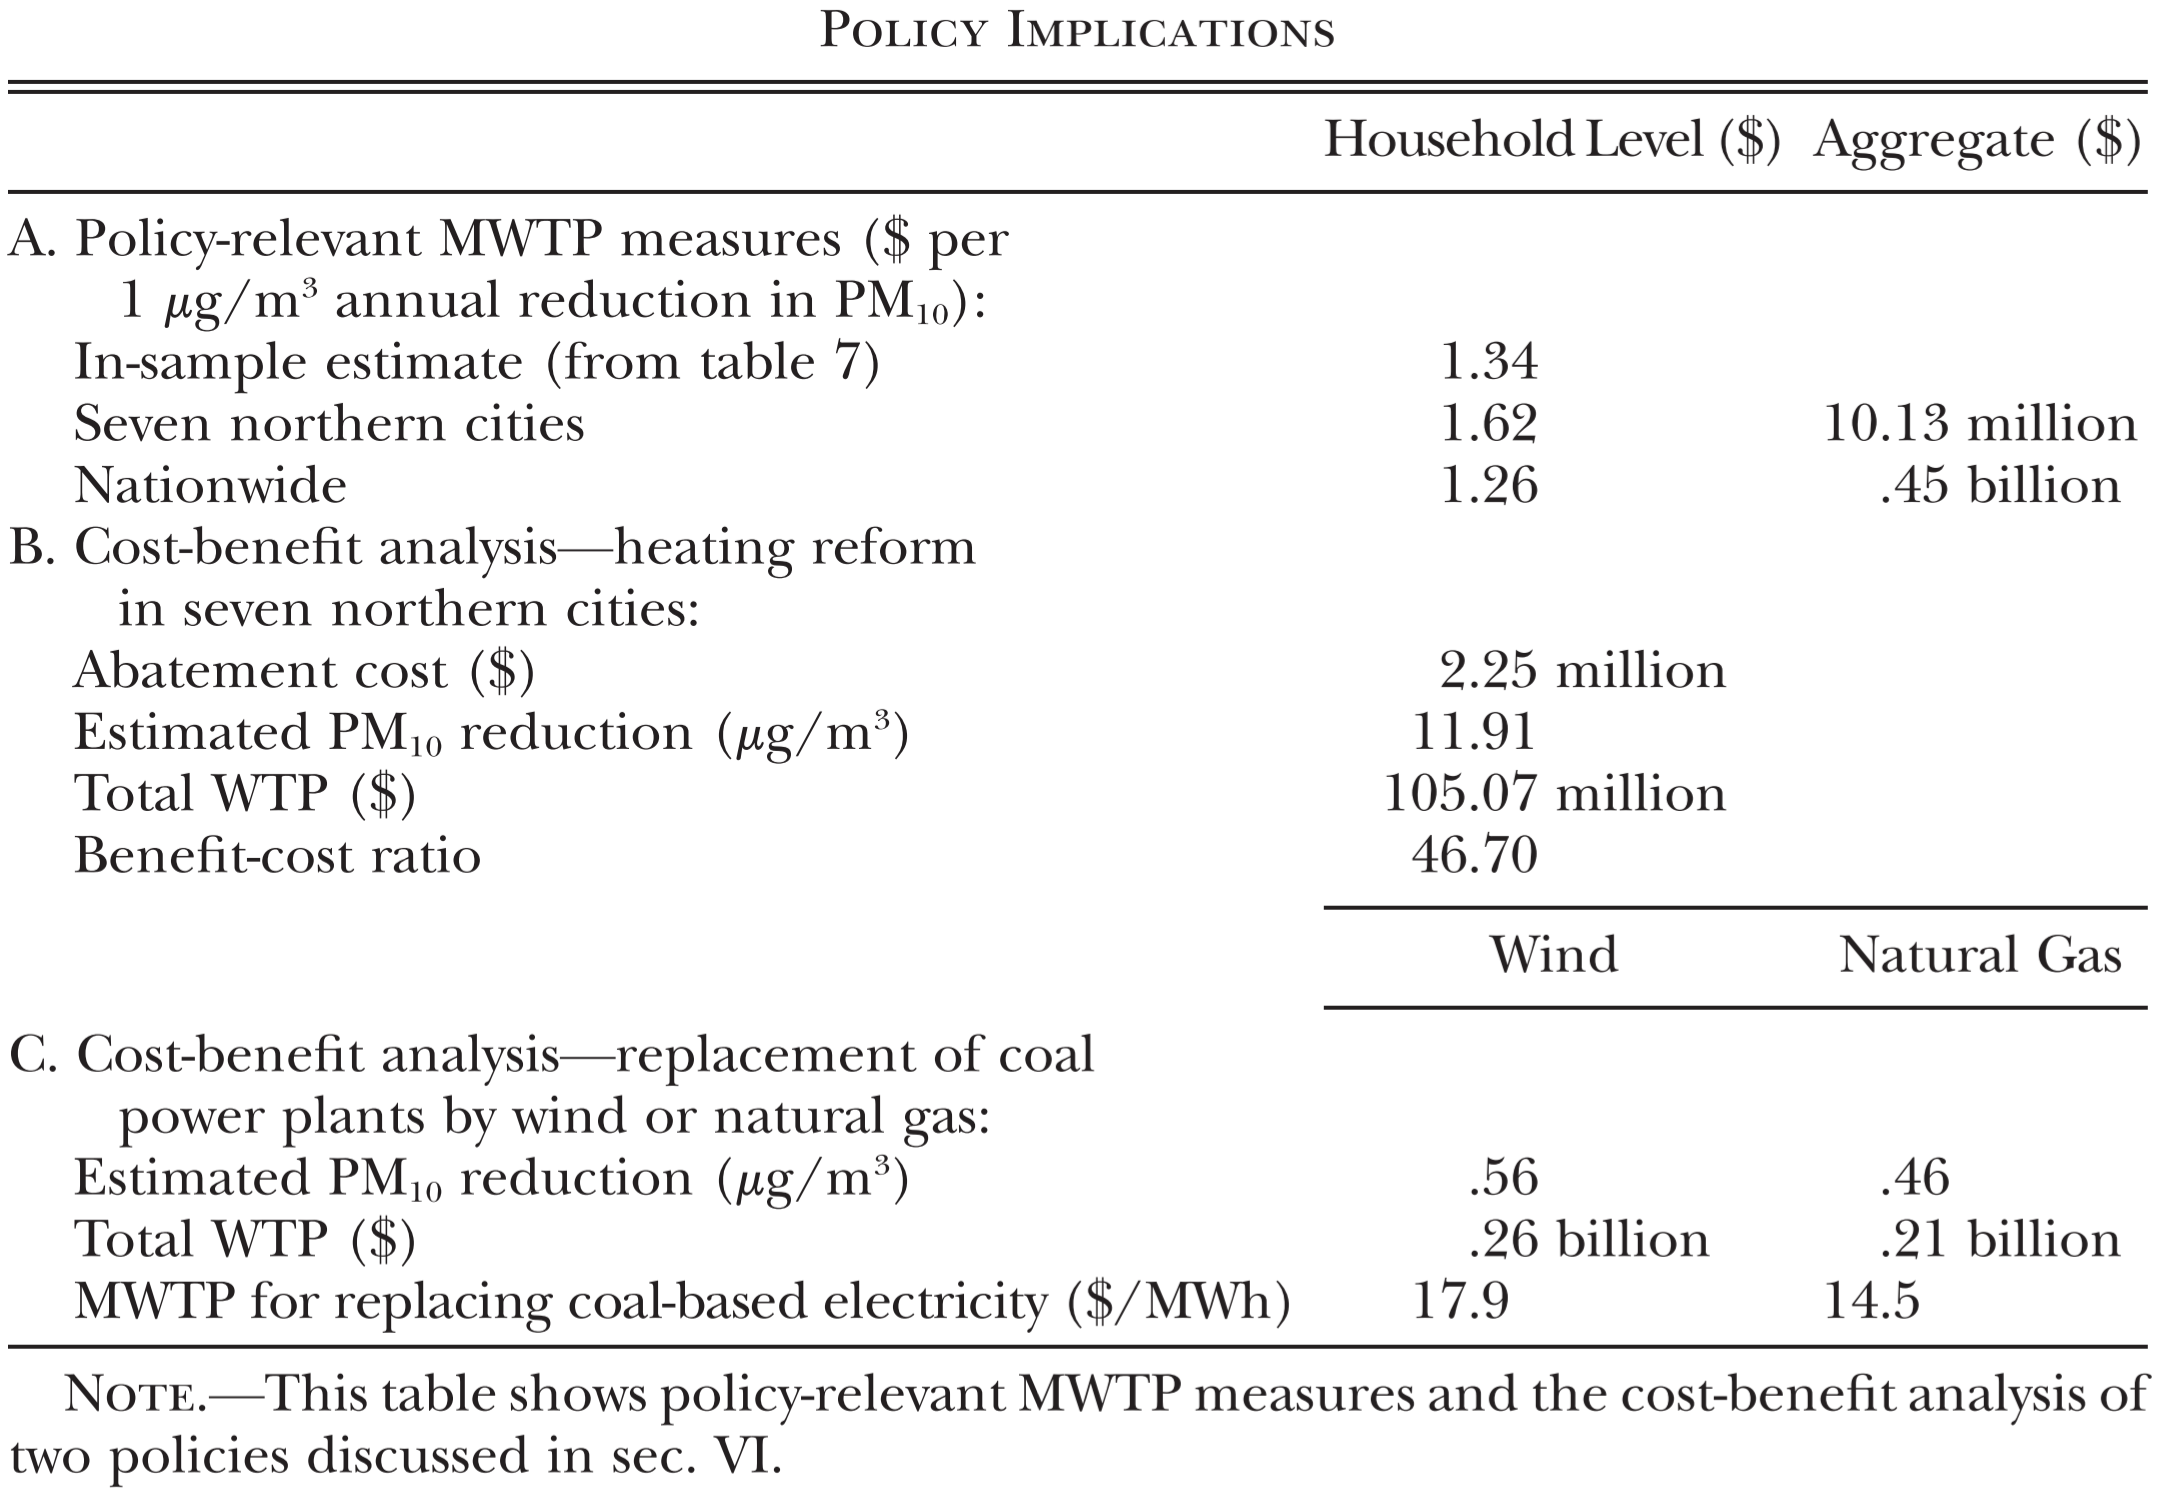
\includegraphics[scale=0.35]{table8.png}	
\end{frame}
%------------------------------------------------
\begin{frame}{E. Heterogeneity in WTP for Clean Air}
	\centering
	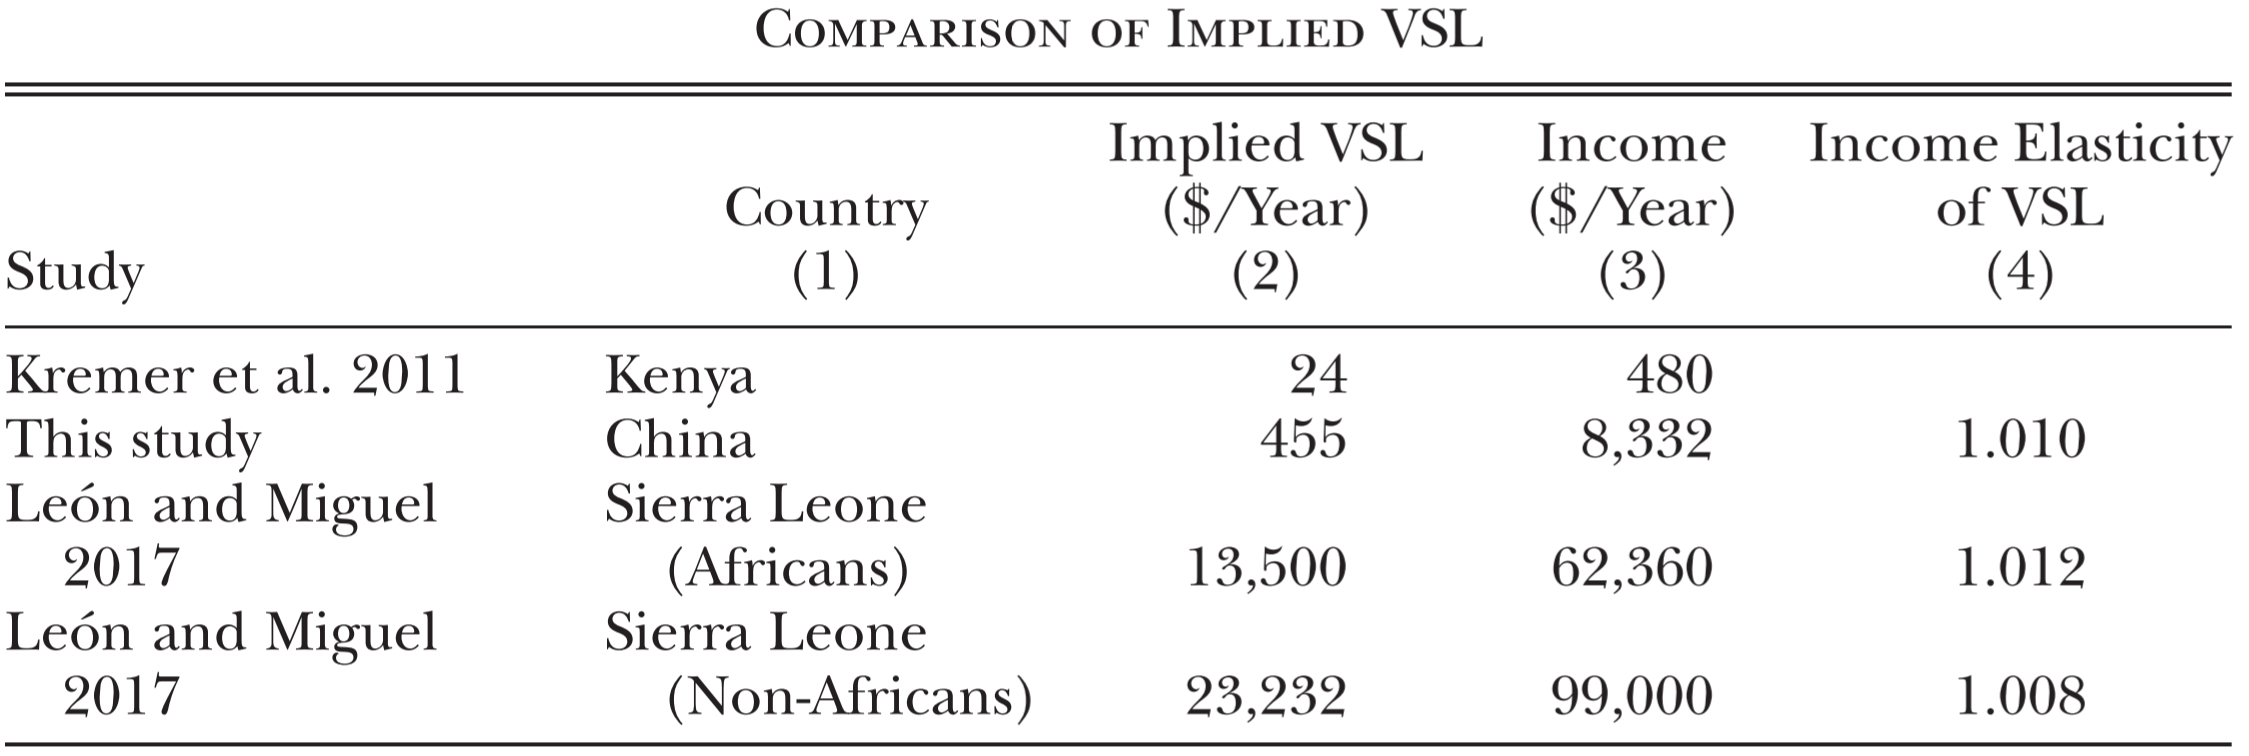
\includegraphics[scale=0.35]{table9.png}	
\end{frame}
%------------------------------------------------






%------------------------------------------------
\section{Limitations \& Further Work}
\begin{frame}[shrink]
	\transfade %fade in and fade out
	\tableofcontents[sectionstyle=show/shaded,subsectionstyle=show/shaded/hide]
	\addtocounter{framenumber}{-1}
\end{frame}
%------------------------------------------------
\begin{frame}{Limitations \& Further Work}
	\begin{itemize}
		\item First, a limitation of our data set is that we do not observe individual-level transactions.
		\item [-] It needs to be assumed that a household can purchase at most one air purifier and uses it for 5 years on average.
		\item [-] The data set does not include online sales.
		\item Second, there is no information on indoor avoidance behavior besides air purifier purchases.
		\item Third, this paper focuses on a static demand model without exploiting time series variation in the data because the exogenous variation in air pollution comes from cross section.
		\item Fourth, there needs to be more research on how market failures affect revealed-preference estimates of MWTP for environmental quality as emphasized by Greenstone and Jack (2013).

	\end{itemize}
\end{frame}
%--------------

%------------------------------------------------

\begin{frame}
\Huge{\centerline{\textit{The End}}}
\end{frame}
%----------------------------------------------------------------------------------------


\end{document} 